\documentclass[letterpaper, preprint]{aastex}
\usepackage{amsmath, amsfonts, bbm, bm, calc}
\usepackage{graphicx}
\usepackage[normalem]{ulem}

%\usepackage[pdftex]{graphicx}
%\usepackage{epstopdf}
\newcounter{address}
\usepackage{color}
\newcommand{\latin}[1]{\emph{#1}}
\newcommand{\etal}{\latin{et\,al.}}
\newcommand{\ie}{\latin{i.\,e.}}
\newcommand{\eg}{\latin{e.\,g.}}
\newcommand{\unit}[1]{\mathrm{#1}}


\definecolor{red}{rgb}{1,0,0}
\definecolor{blue}{rgb}{0,0,1}
\definecolor{darkgreen}{rgb}{0,0.5,0}

%  Display a comment in red, for discussion in drafts
%  To make the comments go away, uncomment the second version of the command

\newcommand{\qer}[1]{{\color{red}#1}}
%\renewcommand{\qer}[1]{}     %  Uncomment this to make the red comments go away.

\usepackage{hyperref}


\begin{document}
\title{
  Diffusive Nested Ensemble Sampling
}

\begin{abstract}
Diffusive Nested Sampling proves to be an efficient and most importantly accurate method to evaluate bayesian evidence integral. We developed an affine invariant ensemble version of the Diffusive Nested Sampling Method to evaluate bayesian evidence integral. We tested our code on models whose evidences can be calculated analytically and got satisfactory results. As an example, we also evaluate different models' evidence integrals of exoplanet radial velocity fitting for 'star 122' and confirm that 2-companion model fitting has the largest evidence.

\end{abstract}

\keywords{
methods: nested sampling
---
methods: markov chain monte carlo
---
methods: data analysis
---
bayesian decision theory
}

\section{Introduction}

In bayesian decision theory, one should return the best mixture of competing models instead of simply deciding which model is the best. To achieve this, the evaluation of evidence integral $Z$ is required. Bayesian decision theory can be summarized as
\begin{equation}
P(\mathrm{Model}_j|\mathrm{Data})=\frac{P(\mathrm{Data}|\mathrm{Model}_j)P(\mathrm{Model}_j)}{\sum_j{P(\mathrm{Data}|\mathrm{Model}_j)P(\mathrm{Model}_j)}},
\label{eq:bayesian-decision-theory}
\end{equation}
which is just the Bayes law. The \textit{likelihood} in Eqn. (\ref{eq:bayesian-decision-theory}) is in fact the evidence $Z_j$ for model j.
\begin{equation}
Z_j=P(\mathrm{Data}|\mathrm{Model}_j)=\int P(\mathrm{Data}|\theta, \mathrm{Model}_j) P(\theta|\mathrm{Model}_j)\mathrm{d}\theta,
\end{equation}
where $P(\mathrm{Data}|\theta, \mathrm{Model}_j)$ is the likelihood of parameter $\theta$ for model j and $P(\theta|\mathrm{Model}_j)$ is the prior of parameter $\theta$ for model j. To make notations simple, we will use $L(\theta)$ for the likelihood and $\pi(\theta)$ for the prior. We'll also drop the index $j$ in $Z_j$ because the discussion applies to all models. So the evidence can be written as
\begin{equation}
Z=\int\! L(\theta)\pi(\theta)\mathrm{d}\theta.
\end{equation}
The prior $\pi(\theta)$ is normalized in the parameter space, that is
\begin{equation}
\int\!\pi(\theta)\mathrm{d}\theta=1,
\end{equation}
while the likelihood $L(\theta)$ is not.

However, evaluating or even estimating the evidence integral has always been challenging. Diffusive Nested Sampling proves to be an efficient and accurate method to evaluate or estimate the evidence \citep{brewer11a}. We hope to take advantage of affine invariant ensemble sampler \citep{goodman10a} to make diffusive nested sampling even more efficient.


\section{Diffusive Nested Sampling}

In nested sampling, we change the variable in the evidence integral from parameter $\theta$ to the prior mass
\begin{equation}
M(L^*)=\int_{L(\theta)>L^*}\!\pi(\theta)\mathrm{d}\theta,
 \label{eq:prior-mass}
\end{equation}
which is, in another word, cumulant prior mass covering the area whose likelihood values are greater than $L^*$ \citep{skilling06a}. $M$ is a monotonically decreasing function of $L^*$ and it ranges from 0 to 1. And the mapping between $M$ and $L^*$ is a bijection. An infinitesimal increment of $M$ is
\begin{equation}
\mathrm{d}M=\int_{L^*-\mathrm{d}L^*<L(\theta)<L^*}\!\pi(\theta)\mathrm{d}\theta = \pi(\theta)\times \mathrm{volume\,of}\,\theta,\,\mathrm{satisfying}\, L^*-\mathrm{d}L^*<L(\theta)<L^*.
\end{equation}
Multiply both sides with $L^*$ and integrate. It is easy to see that
\begin{equation}
\int^1_0\! L^*\mathrm{d}M=\int\!L(\theta)\pi(\theta)\mathrm{d}\theta.
\end{equation}
so evidence $Z$ can be expressed as
\begin{equation}
Z=\int^1_0\! L^*(M)\mathrm{d}M.
 \label{eq:evidence-prior-mass}
\end{equation}
So the integral $Z$ is the area below the $L^*(M)$ curve. In most cases, it is impossible to know the function $L^*(M)$ analytically and evaluate the integral analytically. Note from Eqn. (\ref{eq:evidence-prior-mass}) that $M$ can be viewed as a random variable with uniform distribution. Nested sampling takes advantage of this and proposes to build the $L^*(M)$ curve statistically.

\subsection{Level and Constrained Prior}
In nested sampling, we first try to find several points on the $L^*(M)$ curve, $\{(M_0, L_0^*),(M_1,L_1^*),\ldots\}$. We call these points levels. The $L^*$ is called a level's likelihood threshold or just threshold. Each level defines a constrained prior,
\begin{equation} 
p_{L_j^*}(\theta) = \frac{\pi(\theta)}{M_j}\mathbbm{1}_{L(\theta)>L_j^*},
\label{eq:constrained-prior}
\end{equation}
where
\begin{eqnarray*}
\mathbbm{1}_{L(\theta)>L_j^*} &=& 1,\,\,L(\theta)>L_j^*,\\
& &0,\,\,\mathrm{otherwise},
\end{eqnarray*}
and note that $p_{L_j^*}$ is properly normalized by $M_j$. 

\subsection{Setting Level Thresholds}
We already know the right-most point on the curve, $\left(M_0 = 1,\,L_0^*=0\right)$, which is level 0, because there is no restriction on the likelihood function with $L_0^*=0$ and from the definition of prior mass, Eqn. (\ref{eq:prior-mass}), $M(\theta)$ should cover the whole parameter space. And most likely another point on the left-most side of the curve, $\left(M_{max}=0,\,L_{max}\right)$.

To find the first level $\left(M_1, \,L^*_1\right)$, we generate $N$ samples from the prior density $\pi(\theta)$, $\theta_1$, $\ldots$, $\theta_N$. We calculate the likelihoods $L(\theta_k)$.  We choose $L^*_1$ so that the number of $k$ with $L(\theta_k) > L^*_1$ is $N/e$. A better way to do this is with the algorithm called {\bf quick find}. In the STL it is described here: \href{http://www.cplusplus.com/reference/algorithm/nth_element/}
{\color{blue} \bf \tt /http://www.cplusplus.com/reference/algorithm/nth\_element/}. $M_1\approx1/e$ is the prior mass that level 1 covers (the prior mass of the parameters whose likelihoods are larger than $L_1^*$). $M_1$ is a random variable and its expectation and variance will be given below. 

One way to estimate the next level $\left(M_2, \,L^*_2\right)$ would be to generate $N$ samples from  the constrained prior density $p_{L_1^*}(\theta)$ defined in Eqn. (\ref{eq:constrained-prior}). But instead, we generate samples from a mixture of $p_{L_1^*}(\theta)$ and prior $\pi(\theta)$ until we have $N$ samples with likelihood larger than  the previous level's threshold $L_1^*$. We sample the mixture because the area covered by level 1 may be disconnected in paremeter space and only sampling the constrained prior $p_{L_1^*}(\theta)$ may get us stucked in only one or few of those disconnected areas. Like before, we get a chain of $N$ likelihoods, rank these likelihoods in descending order and find the $N/e$-th likelihood, which we call $L_2^*$. This would give us another point on the $L^*(M)$ curve, which is approximately $(1/e^2,L_2^*)$. This is level 2 and $L_2^*$ is the likelihood threshold of level 2. Again, $M_2\approx1/e^2$ is the prior mass that level 2 covers. Like $M_1$, $M_2$ is also a random variable. The variance of $M_1$ and $M_2$ ca be calculated by using order statistics.

There is a simple stopping criterion to tell how many levels are enough. Suppose we already have levels $\left(M_1,\,L^*_1\right), \ldots, \left(M_k,\,L^*_k\right)$. The evidence integral corresponding to all these levels is
$$
Z_k = \sum_{j=0}^{k-1} \int_{M_j}^{M_{j+1}} L^*(M)\mathrm{d}M 
$$
The remaining integral is
$$
\int_{M_k}^1 L^*(M) \mathrm{d}M \; .
$$
But $L^*(M) < L_{max}$ always, so the remain integral cannot be larger than $L_{max}(1-M_k)$. We choose a stopping point $k$ so that $L_{max}(1-M_k) \leq \epsilon Z_k$. We usually choose $\epsilon = 10^{-6}$.

At the end, we get a series of points on the $L^*(M)$ curve, $\{(M_0, L_0^*),(M_1,L_1^*),(M_2,L_2^*), \ldots\}$. Correspondingly, we also have a series of mixture of constrained priors,
\begin{equation}
p(\theta) = \sum_{j=0} w_j p_{L_j^*},
\label{eq:mixture-constrained-prior}
\end{equation}
where $p_{L_j^*}$ is the constrained prior defined by level $j$,
\begin{equation} 
p_{L_j^*}(\theta) = \frac{\pi(\theta)}{M_j}\mathbbm{1}_{L(\theta)>L_j^*},\,\,\,j=0,1,2,\ldots.
\end{equation}
and $w_j$ are the weights of each level which sum up to 1,
\begin{equation}
\sum_{j=0}w_j = 1.
\end{equation}
The choice of weight may change according to different purposes. For example, when we are building a new level, we might want to put more weight on the last level. And in the final stage, when we sample all the levels together, we might want to have the same weight on all the levels.

\subsection{Affine Invariant Stretch Move}
To implement the affine invariant ensemble sampler to diffusive nested sampling, we assign different levels to different walkers in the ensemble. This probably would cause concern since all the walkers would be from different density and this might render stretch move invalid. But in the stretch move, the helper walker does not interfere with the walker which it helps, even if they are from different density distribution. 

Our goal is to sample the mixture of the constrained priors Eqn. (\ref{eq:mixture-constrained-prior}). We realize it by updating the walkers according to their own constrained priors Eqn. (\ref{eq:constrained-prior}) and updating the indices of the levels of those walkers according to their weights and other restrictions. So the algorithm consists of two part: updating the ensemble of walkers followed or preceded by updating all the level indeces of those walkers. The first part can be summarized as:
\qer{JG: probably $X_{new} = \cdots$, and $\alpha=z$.  I don't think the 
metropolis part is stated correctly.} \qer{FH: It should be correct now.}
\begin{sffamily}
\begin{itemize}
\item randomly choose a helping walker $Y$
\item propose a new walker with stretch move: $X_{new} \rightarrow Y + \alpha (X_{old}-Y)$, where $\alpha$ is a random variable from some distribution \citep{goodman10a}.
\item if the proposed $X_{new}$ has a likelihood smaller than its current threshold $L^*$, reject the proposal.
\item else, accept the proposed $X_{new}$ with probability: $\mathrm{max}\left(z^{\mathrm{dim}-1}\frac{p_{L^*}(X_{new})}{p_{L^*}(X_{old})},1\right)$.
\end{itemize}
\end{sffamily}
The second part can be summarized as \citep{brewer11a}:
\begin{sffamily}
\begin{itemize}
\item propose a new level for a walker in the ensemble, with proposal probability, Eqn. (\ref{eq:index-proposal-prob}): $i \rightarrow j$
\item if $j \geq i$, accept the proposal if, in parameter space, the likelihood of the walker is larger than $L_j^*$; reject if it is smaller.
\item else, accept the proposal with probability $\mathrm{min}\left(\frac{M_i}{M_j}\frac{w_j}{w_i},1\right)$.
\end{itemize}
\end{sffamily}
The proposal probabilities for the second part, $T_{i\rightarrow j}$, can be written as entries of matrix $T$,
\begin{equation}
(T_{i\rightarrow j}) = (T_{ij})
\begin{pmatrix}
0.5 & 0.5 & & & & & \\
0.5 & 0 & 0.5 & &  & & \\
 & 0.5 & 0 & 0.5 &  &  & \\
 &  & \ddots & \ddots & \ddots  &  & \\
 &  &  &  0.5 &  0 & 0.5 &  \\
 &  &  &  &  0.5 & 0 & 0.5 \\
 &  &  &  &  & 0.5 & 0.5 \\
\end{pmatrix}
\label{eq:index-proposal-prob}
\end{equation}

\subsection{Refining Level Masses}
Constructing levels and sampling a mixture of constrained priors $p(\theta),$ Eqn. (\ref{eq:mixture-constrained-prior}), are equivalent to finding a probability density function $p(\theta)$ similar in shape with $L(\theta)\pi(\theta)$ and performing importance sampling. We can refine the prior masses $M$'s of the levels to have a more accurate $p(\theta)$ and thus a more accurate importance function $\frac{L(\theta)\pi(\theta)}{p(\theta)}$.

Suppose we have $J$ levels, $\{(M_1,L_1^*),(M_2,L_2^*), \ldots,(M_J,L_J^*)\}$. Sampling the mixture of constrained priors Eqn. (\ref{eq:mixture-constrained-prior}), we can refine the prior masses $\{M_1,\dots,M_J\}$ by keeping track of all the levels the walkers have visited as well as the likelihoods of those visits . Assuming the sampler has visited level $j-1$ for $n_{j-1}$ times and during those $n_{j-1}$ visits there are $n_{j-1}^j$ times that the likelihoods exceed level $j$'s threshold $L^*_j$, we can refine $M_j$ as following \citep{brewer11a}
\begin{equation}
M^*_j = M^*_{j-1}\frac{n_{j-1}^j+C M_j/M_{j-1}}{n_{j-1}+C},
\end{equation}
where $M^*$'s are the refined prior masses and $C$ is a constant that reflects one's confidence in the accuracy of the levels before this refinement. We use $C=10^4$. Of course $M^*_0=1$ and we starts from refining $M_1$, so $M^*_{j-1}$ will be known when we refine $M_j$. If $n_{j-1}$ and $n_{j-1}^j$ dwarf $C$, the variance of $M^*_j$ is approximately
\begin{equation}
\mathrm{var}\left(\frac{M^*_j}{M^*_{j-1}}\right)\approx\frac{1/e(1-1/e)}{n_{j-1}}.
\end{equation}

While sampling the mixture of constrained priors Eqn. (\ref{eq:mixture-constrained-prior}), it is possible that the weights $w_j$ are not sampled as desired. This happens when the prior masses of levels are not estimated accurately. As a result, the acceptance probability $\mathrm{min}\left(\frac{M_i}{M_j}\frac{w_j}{w_i},1\right)$ deviates from desired. Paradoxically, We need the weights to be sampled as desired in order to refine the prior masses to be more accurate. In such cases, we can implement certain reinforcing mechanism. \citep{brewer11a}

\subsection{Computing Evidence}
We take the mean of likelihoods sandwiched between two levels,
\begin{equation}
\bar{L}_j= \frac{1}{n_j}\sum_{L_j^*\leq L(\theta)<L_{j+1}^*} L(\theta),
\end{equation}
where $\theta$ represents samples. Again with the extra level whose likelihood threshold $L^*_{J+1}$ is the maximum likelihood and prior mass $M_{J+1}$ is 0, the evidence is
\begin{equation}
Z = \sum_{j=0}^{J} \bar{L}_j (M^*_j - M^*_{j+1}).
\end{equation}


\section{2-d Gaussian Testing Case}
The algorithm was tested on a 2-d gaussian likelihood and a 2-d uniform prior. The likelihood is
\begin{equation}
L(\theta_1,\theta_2)=\frac{1}{2\pi\sigma^2}\exp{\left(-\frac{\theta_1^2+\theta_2^2}{2\sigma^2}\right)},\;\sigma = 1,
\label{eq:likelihood2}
\end{equation}
where $\theta_1$ and $\theta_2$ are the parameters. The prior is
\begin{equation}
\pi(\theta_1,\theta_2) = \frac{1}{400},\;\theta_1\in[-10,\,10],\;\theta_2\in[-10,\,10],
\label{eq:prior2}
\end{equation}
and 0 otherwise. This prior basically is a square whose sides' length is 20 and whose area is 400. The evidence is approximately inverse of that area,
\begin{equation}
\mathrm{evidence} \approx \frac{1}{400},
\end{equation}
where the approximation is equivalent to equality up to machine error because gaussian distribution has extremely thin tail. The likelihood threshold of any level can be analytically calculated in this model. As a matter of fact, the whole $L^*(M)$ curve can be built analytically,
\begin{equation}
\log{L^*(M)}=-\log{2\pi}-\frac{200M}{\pi},
\label{eq:analytical-threshold}
\end{equation}
where the number $200$ comes from half the area that the prior covers. Note that $\log{L^*}$ is a linear function of $M$.

\subsection{Testing Level Thresholds Setting}
The test is to see if the algorithm can build levels matching the analytically calculated ones. Recall that to find a new level, one needs to generate a chain of $N_1$ likelihoods larger than previous level's threshold. ($N_1$ is used so not to be confused with $N_2$ used later.) Each new level requires $N_1$ likelihoods. Two $N_1$'s are tested, $N_{1a} = 10,000$ and $N_{1b} = 100,000$. The larger $N_{1b}$ should give a smaller variance than $N_{1a}$. For both $N_{1a}$ and $N_{1b}$, 6 levels are built  for $10,000$ times in order to check the statistical features of these levels.

For $N_{1a} = 10,000$, after ranking the chain of $N_{1a}$ likelihoods in descending order, the $J_{1a} = 3,678$-th likelihood is picked as the new level's threshold. For $N_{1b} = 100,000$, after ranking the chain of $N_{1b}$ likelihoods. the $J_{1b} = 36,787$-th likelihood is picked as the next level's threshold. 

For $N_{1a}$, the expectation of the prior masses that each level covers are $\left\{\frac{J_{1a}}{N_{1a}+1},\left(\frac{J_{1a}}{N_{1a}+1}\right)^2,\ldots\right\}$. And for $N_{1b}$, the expectation of the prior masses that each level covers are $\left\{\frac{J_{1b}}{N_{1b}+1},\left(\frac{J_{1b}}{N_{1b}+1}\right)^2,\ldots\right\}$. The variance of the prior masses can also be easily calculated. For example, the variance of the 1st level's covered mass is $\frac{(J_{1a})(N_{1a}-J_{1a})}{(N_{1a}+1)^2(N_{1a}+2)}$ for $N_{1a}$ and $\frac{(J_{1b})(N_{1b}-J_{1b})}{(N_{1b}+1)^2(N_{1b}+2)}$ for $N_{1b}$. The expection and variance of the corresponding (logarithm of) likelihood thresholds can then be calculated straightfowardly, because $\log{L^*}$ is a linear fuction of $M$ (from Eqn. (\ref{eq:analytical-threshold})). The mean values of the 6 levels' thresholds are listed in Tab. (\ref{tab:threshold-mean}) for both $N_{1a}$ and $N_{1b}$ together with the corresponding analytical values of the thresholds. The standard deviations with their analytical values are listed in Tab. (\ref{tab:threshold-variance}). The histograms of level1 and level 6 are visualized in Fig. (\ref{fig:level1-6})


\subsection{Testing Constrained Prior Mixture}
We draw samples from a mixture of all the constrained priors defined by true levels listed in Tab. (\ref{tab:true-levels}). Every adjacent two levels define a bin. For each sample, we find two adjacent levels whose thresholds sandwich the likelihood of the sample and that sample can be put into the bin defined by those two levels. The prior masses of samples inside each bin should follow uniform distribution, which is consistent with our testing result, illustrated in Fig. (\ref{fig:hist-gaps}). The variances of the likelihoods of samples can vary dramatically among different bins, Fig. (\ref{fig:level-var}).

\section{High-Dimension Gaussian Testing Case}

In 10-d case, the likelihood is
\begin{equation}
L(\boldsymbol{\theta})=\frac{1}{(2\pi\sigma^2)^{10/2}}\exp{\left(-\frac{\boldsymbol{\theta}^2}{2\sigma^2}\right)},\;\sigma = 1,
\label{eq:likelihood10}
\end{equation}
where $\theta_1$ and $\theta_2$ are the parameters. The prior is
\begin{equation}
\pi(\boldsymbol{\theta}) = \frac{1}{20^{10}},\;\theta_j\in[-10,\,10],\;j=1,2,\ldots,10,
\label{eq:prior10}
\end{equation}
and 0 otherwise. We make 30 levels in 10-d case so that the last level will cover approximately $1/20^{10}$ of the total prior hyper-volume. To build each level, a likelihood chain of length $N_1$ is generated. After all the levels are built, we sample mixture of constrained priors for $N_2$ times, using these samples to refine the prior masses and evaluate the evidence.

\subsection{Testing Prior Mass Refinement}
We repeat the prior mass refinement and evidence evaluation for $1,000$ times for different $N_1$'s and $N_2$'s. The mean evidences for all $N_1$'s and $N_2$'s are very close to the true evidence  $9.77\times10^{-14}$. The standard deviations are summarized in Tab. (\ref{tab:N1N2}).

\section{Exoplanet for Star 122}
Star 122 has two confirmed companions (citation). We fit the radial velocity data of Star 122 with 1-companion, 2-companion and 3-companion model and evaluate the evidence integrals for these models to see if the 2-companion model has a larger evidence than the other two.

For simplicity, uniform priors are used. For the 5 orbital parameters, the priors are
\begin{align}
\pi(A) &= \frac{1}{10000}\,\unit{(m\,s^{-1})^{-1}},&&A\in[0,10000]\,\unit{m\,s^{-1}},\\
\pi(\omega) &= 1\,\unit{(rad\,d^{-1})^{-1}}, &&\omega\in[0,1]\,\unit{rad\,d^{-1}},\\
\pi(\phi) &= \frac{1}{2\pi}\,\unit{rad^{-1}},&&\phi\in[0,2\pi]\,\unit{rad},\\
\pi(e) &= 1,&&e\in[0,1],\\
\pi(\varpi) &= \frac{1}{2\pi}\,\unit{rad^{-1}},&&\varpi\in[0,2\pi]\,\unit{rad}.
\end{align}
The offset and jitter have priors
\begin{align}
\pi(v_0) &= \frac{1}{10000}\,\unit{(m\,s^{-1})^{-1}},&&v_0\in[-5000,5000]\,\unit{m\,s^{-1}},\\
\pi(s^2) &=\frac{1}{100000}\,\unit{(m^2\,s^{-2})^{-1}},&&s^2\in[0,100000]\,\unit{m^2\,s^{-2}}.
\end{align}
We do not include linear trend as a parameter because there is clearly a massive long-period companion whose period can be fitted very accurately.

The optimal-fit parameters for 1-companion, 2-companion and 3-companion models are summarized in Tab. (\ref{tab:best-fit-star-122}). The fits are shown in Fig. (\ref{fig:fit-122-1-2-3}) and Fig. (\ref{fig:fit-122-2-3-zoom}). The evidence of 1-companion model is $\exp{(-486.4139\pm0.0434)}$. The evidence of 2-companion model is $\exp{(-399.9947\pm0.0848)}$. The evidence of 3-companion model is $\exp{(-403.7936\pm0.1604)}$. The levels of these models are shown in Fig. (\ref{fig:levels-122}). So the 1-companion model is extremely unlikely. And 2-companion model is about 44 times more likely than the 3-companion model.

\begin{table}[h]
\centering
\begin{tabular}{l|l|l|l}
 & 1-companion model & 2-companion model & 3-companion model\\
\hline
log likelihood & -446.054 & -322.223 & -314.403\\
\hline
$A_1\,(\unit{m\,s^{-1}})$ & $4036.14$ & $4016.07$ & $4015.09$\\
$\omega_1\,(\unit{rad\,d^{-1}})$ & $4.87235\times10^{-4}$ & $5.24207\times10^{-4}$ & $5.16891\times10^{-4}$\\
$\phi_1\,(\unit{rad})$ & $4.68676$ & $4.56655$ & $4.59078$\\
$e_1$ &  $0.745968$  & $0.734338$  & $0.736879$\\
$\varpi_1\,(\unit{rad})$ & $4.16403$ & $4.17599$ & $4.17536$\\
\hline
$A_2\,(\unit{m\,s^{-1}})$ &  & $134.792$ & $132.058$\\
$\omega_2\,(\unit{rad\,d^{-1}})$ &  & $0.0210239$ & $0.0210218$\\
$\phi_2\,(\unit{rad})$ &  & $5.39148$ & $5.37908$\\
$e_2$ & & $0.0503521$ & $0.0370734$\\
$\varpi_2\,(\unit{rad})$ &  & $3.50770$ & $3.53115$\\
\hline
$A_3\,(\unit{m\,s^{-1}})$ &  &  & $12.9190$\\
$\omega_3\,(\unit{rad\,d^{-1}})$ &  &  & $9.64646\times10^{-3}$\\
$\phi_3\,(\unit{rad})$ &  &  & $3.09382$\\
$e_3$ &  &   & $0.366577$\\
$\varpi_3\,(\unit{rad})$ &  &  & $2.38103$\\
\hline
$v_0\,(\unit{m\,s^{-1}})$ & $-234.629$ & $-247.814$ & $-239.267$ \\
$s^2\,(\unit{m^2\,s^{-2}})$ & $8562.04$ & $288.578$ & $251.668$\\
\hline
\end{tabular}
\caption{The optimal-fit parameters for all 3 models are summarized here. The 1st row lists the log likelihoods of the optimal-fit parameters of these 3 models. }
\label{tab:best-fit-star-122}
\end{table}

\begin{thebibliography}

\bibitem[Goodman \etal(2010)]{goodman10a}
Goodman,~J., Weare,~J., 2010, Comm.\ App.\ Math.\ and Comp.\ Sci., 5, 65

\bibitem[Brewer \etal(2011)]{brewer11a}
Brewer,~B.~J., P\'{a}rtay,~L.~B. \& Cs\'{a}nyi,~G, 2011, Statistics and Computing, 21, 649

\bibitem[Skilling (2006)]{skilling06a}
Skilling,~J., 2006, Bayesian Analysis, 4, 833

\end{thebibliography}

\clearpage

\begin{table}[h]
\centering
\begin{tabular}{c|c|c|c|c}
\hline
& \multicolumn{2}{|c|}{$N_{1a}=10,000$} & \multicolumn{2}{|c}{$N_{1b}=100,000$}\\
\hline
Level & experimental mean & analytical value & experimental mean & analytical value\\
\hline
%1 & $-25.2524932657$ & -25.2504110407 &-25.2569110901 & -25.2569744415\\
%2 & $-10.4490276068$ & -10.4481460353 &-10.4529865267 & -10.4529742668\\
%3 & $-5.00537185332$ & -5.00441733912 &-5.00706799218 & -5.00708118148\\
%4 & $-3.00304284678$ & -3.00241412501 &-3.00382130366 & -3.00372052579\\
%5 & $-2.26627087499$ & -2.26615096917 &-2.26679664954 & -2.26675161107\\
%6 & $-1.99543090186$ & -1.99538045751 &-1.99566730020 & -1.99564556747\\
1 & $-25.2525$ & -25.2504 &-25.2569 & -25.2570\\
2 & $-10.4490$ & -10.4481 &-10.4530 & -10.4530\\
3 & $-5.00537$ & -5.00442 &-5.00707 & -5.00708\\
4 & $-3.00304$ & -3.00241 &-3.00382 & -3.00372\\
5 & $-2.26627$ & -2.26615 &-2.26680 & -2.26675\\
6 & $-1.99543$ & -1.99538 &-1.99567 & -1.99565\\
\hline
\end{tabular}
\caption{The experiment was repeated $10,000$ times. The experimental mean values of the logarithm of the 6 levels' thresholds in the table are the mean of the $10,000$ repetitions. Notice that the experimental means for $N_{1b}$ tend to be closer to analytical values than those for $N_{1a}$ as expected.}
\label{tab:threshold-mean}
\end{table} 


\begin{table}[h]
\centering
\begin{tabular}{c|c|c|c|c}
\hline
& \multicolumn{2}{|c|}{$N_{1a}=10,000$} & \multicolumn{2}{|c}{$N_{1b}=100,000$}\\
\hline
Level & experimental std & analytical std & experimental std & analytical std\\
\hline
%1 & 0.362464067018 & 0.306920840463 &0.113447431175 & 0.0970782243791\\
%2 & 0.182170358952 & 0.159635079214 &0.0573525182345 & 0.0505043419815\\
%3 & 0.0813923486799 & 0.0719053024947 &0.0256098683388 & 0.0227544447107\\
%4 & 0.0344988807296 & 0.0305363582783 &0.0107822459632 & 0.00966557076926\\
%5 & 0.0141857964076 & 0.0125562283731 &0.00441558031849 &0.00397534117105\\
%6 & 0.00570328599704 & 0.00505867509443 &0.00177408254067 &0.00160197939064\\
1 & 0.36 & 0.31 &0.11 & 0.097\\
2 & 0.18 & 0.16 &0.057 & 0.051\\
3 & 0.081 & 0.072 &0.026 & 0.023\\
4 & 0.034 & 0.031 &0.011 & 0.0097\\
5 & 0.014 & 0.013 &0.0044 & 0.0040\\
6 & 0.0057 & 0.0051 &0.0018 & 0.0016\\
\hline
\end{tabular}
\caption{The experiment was repeated $10,000$ times. The experimental std of the logarithm of the 6 levels' thresholds in the table are the variance of the $10,000$ repetitions. The algorithm almost achieves the expected precision. Note that the std's for $N_{1a}$ are approximately $\sqrt{10}$ times those for $N_{1b}$.}
\label{tab:threshold-variance}
\end{table} 

\begin{table}[h]
\centering
\begin{tabular}{c|c|c}
\hline
level index & log likelihood threshold & log prior mass\\
\hline
1 & -29.8629798621251 & -1\\
2 & -15.0587589731369 & -2\\
3 & -9.61259046551731 & -3\\
4 & -7.60905703840871 & -4\\
5 & -6.87199828087570  & -5\\
6 & -6.60084951704394 & -6\\
7 & -6.50109946133118 & -7\\
8 & -6.46440346657875 & -8\\
9 & -6.45090376453600  & -9\\
10 &-6.44593750169253 & -10\\
\hline
\end{tabular}
\caption{True levels' thresholds and prior masses are listed in the table. 10 Levels are given. We keep many digits because these are true levels.}
\label{tab:true-levels}
\end{table} 

%\begin{table}[h]
%\centering
%true evidence: $\exp{(-5.991464547107982)}=2.5\times10^{-3}$\\
%\begin{tabular}{c|c|c}
%\hline
%$N$ & evidence mean ($\times10^{-3}$)  & evidence std ($\times10^{-3}$)\\
%\hline
%1,000 & 2.516691134661 & 0.209059516266437\\
%2,000 & 2.507236697647 & 0.146426121804169\\
%3,000 & 2.506617141600 & 0.123673129501314\\
%5,000 & 2.501362156538 & 0.0930265392133242\\
%10,000 & 2.501949543083 & 0.0660132437877751\\
%20,000 & 2.500442865432 & 0.0464402837653896\\
%30,000 & 2.501127417942 & 0.0381871277742115\\
%50,000 & 2.499991370460 & 0.0301503918624074\\
%100,000 & 2.500207281072 & 0.0215658324785832\\
%\hline
%\end{tabular}
%\caption{$N$ is the length of the likelihood chain to build each level. For each different $N$, 10 levels are built. Evidences were evaluated with $1,000,000$ samples from the mixture of the constrained priors, Eqn. (\ref{eq:constrained-prior}). Every experiment is repeated for 10,000 times to evaluate the mean and standard deviation.}
%\label{tab:evi-mean-var}
%\end{table} 

\begin{figure}[h]
 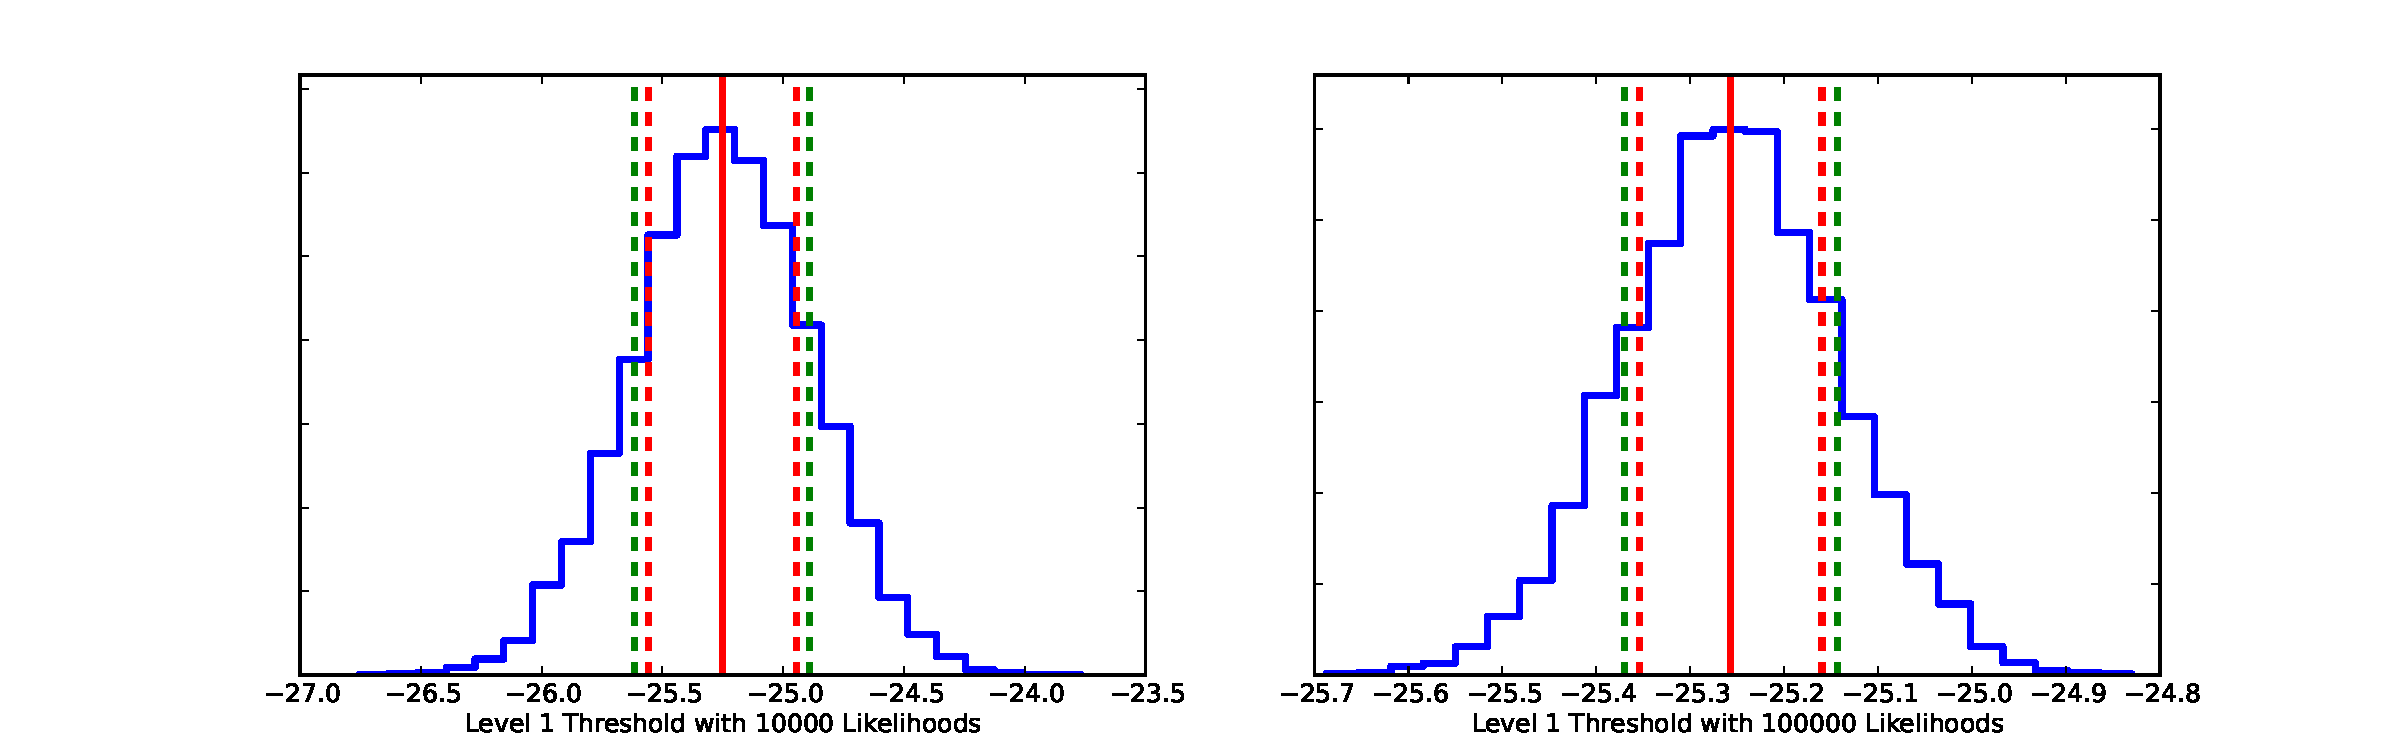
\includegraphics[width=0.99\linewidth]{level1.pdf}\\
 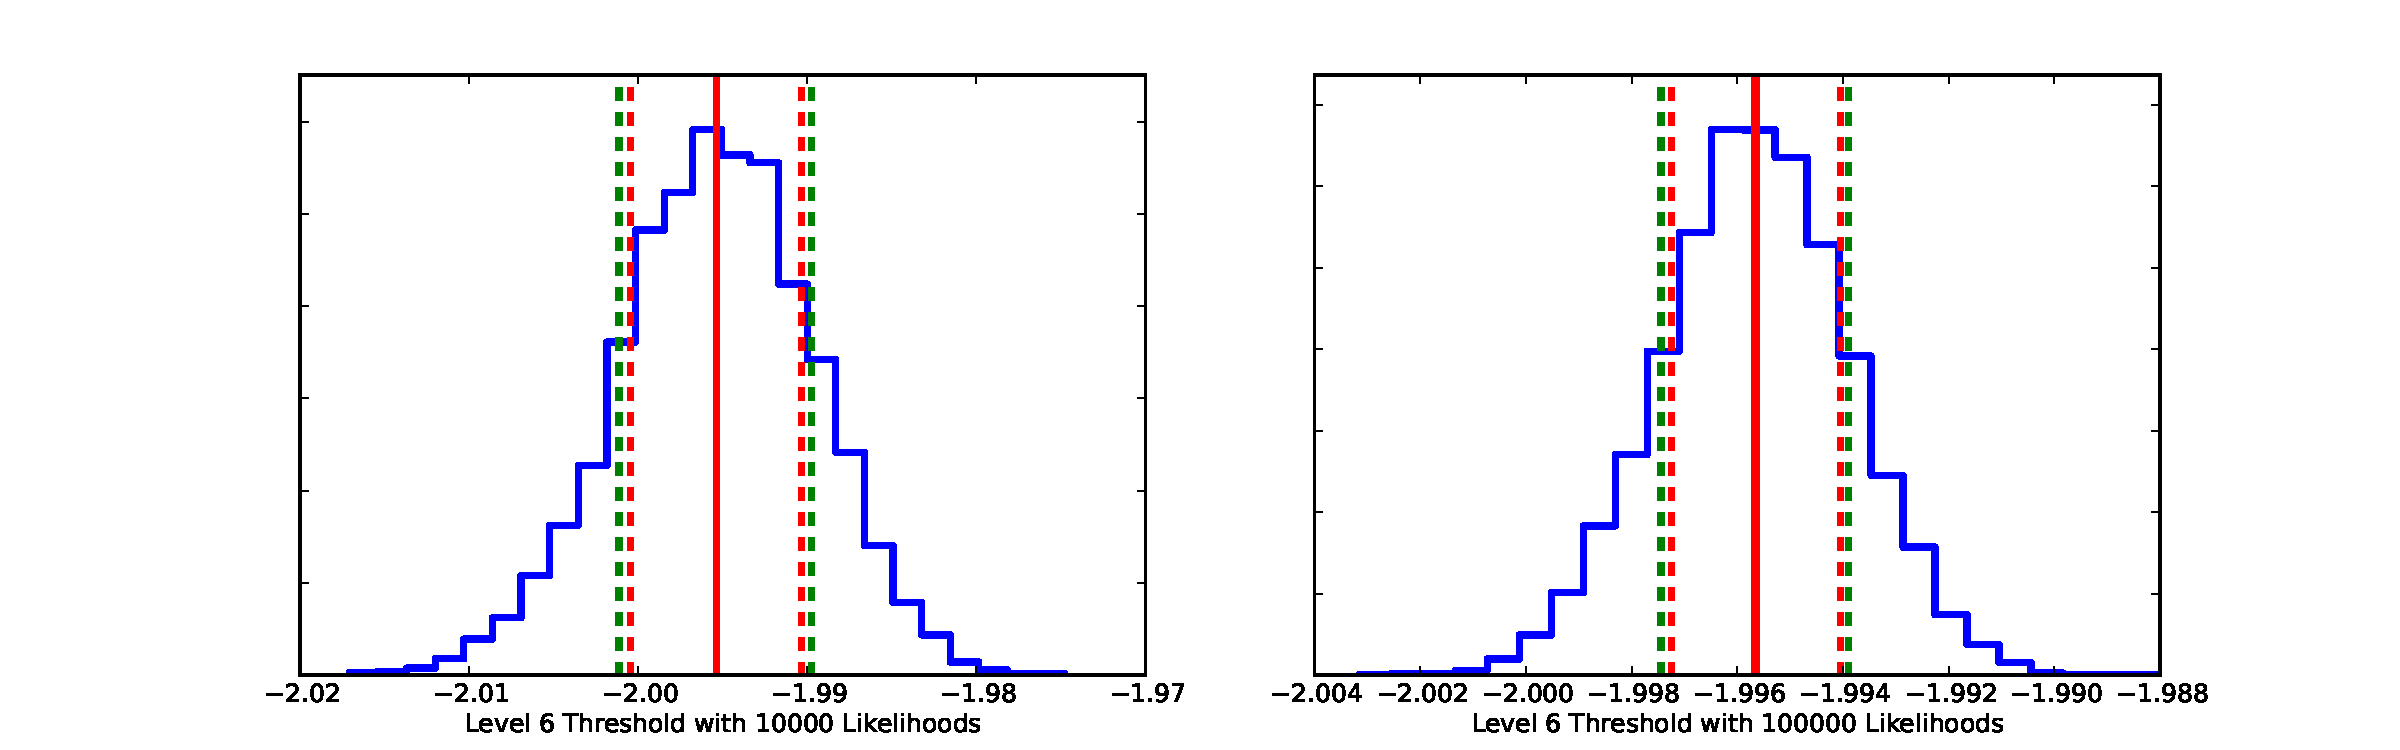
\includegraphics[width=0.99\linewidth]{level6.pdf}
 \caption{Level 1 (upper) and Level 6 (lower): Both histograms are plotted with 25 bins and 10,000 samples. (Here samples mean repetitions of the experiment, not the samples of likelihood to build every single level.) The left-hand side is the histogram of levels built with $N_{1a}$ likelihoods and the right-hand side is the histogram of levels built with $N_{1b}$ likelihoods. The \textcolor{red}{red} solid lines indicate the true values of the logarithm of the likelihood thresholds of levels and \textcolor{darkgreen}{dark green} solid lines indicate the experimental mean of the logarithm of the likelihood thresholds, which cannot be distinguished from the true values in these pictures. The \textcolor{red}{red} dashed lines indicate the theoretical standard deviation and the \textcolor{darkgreen}{dark green} dashed lines indicate the experimental standard deviation.}
 \label{fig:level1-6}
\end{figure}

\begin{figure}[h]
 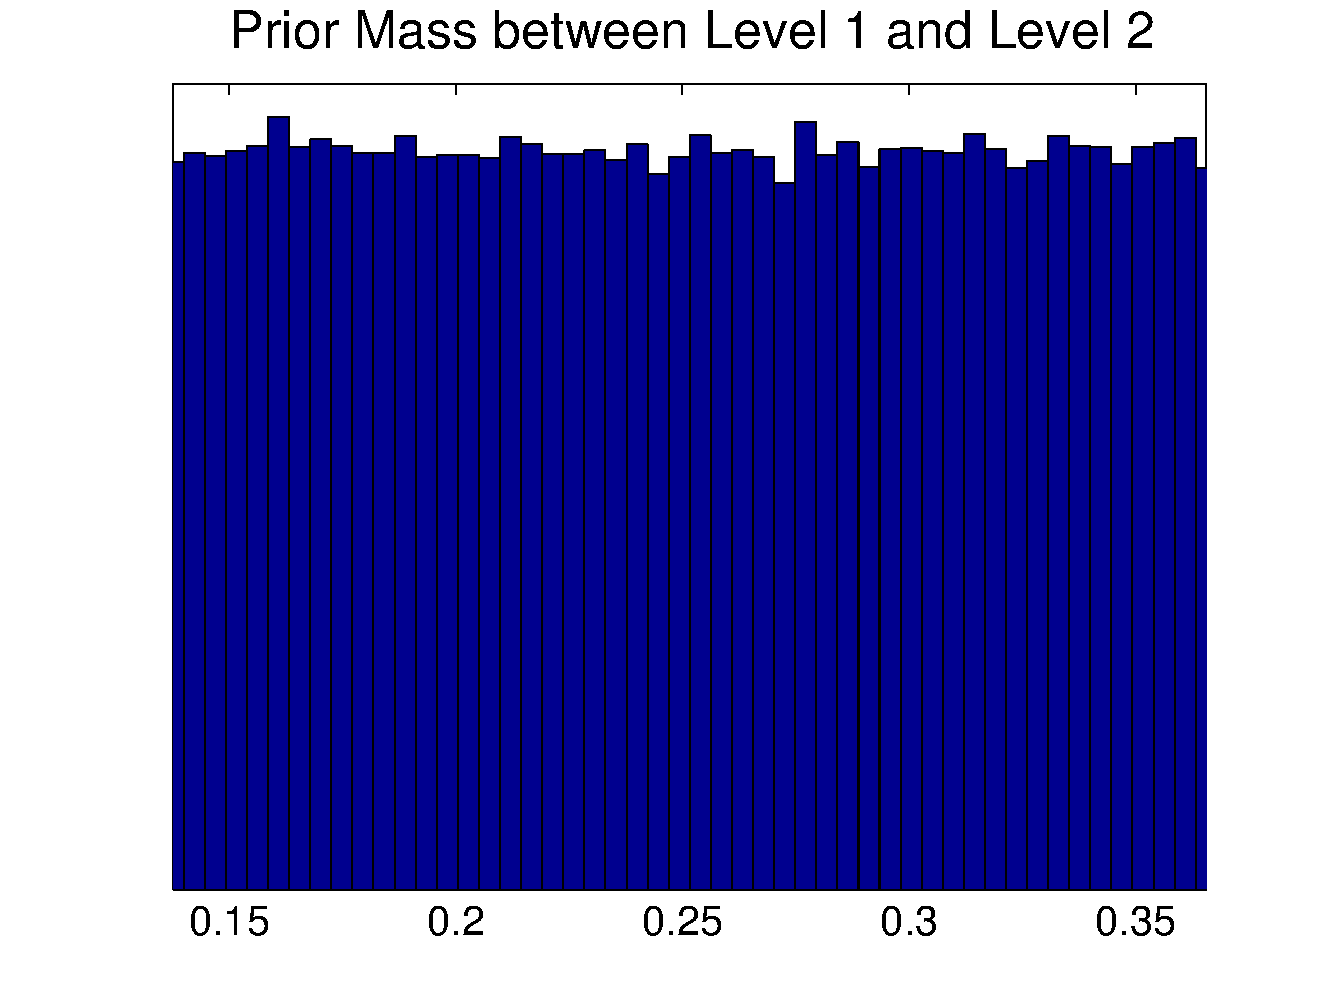
\includegraphics[width=0.45\linewidth]{histgaps-01-02.pdf}
 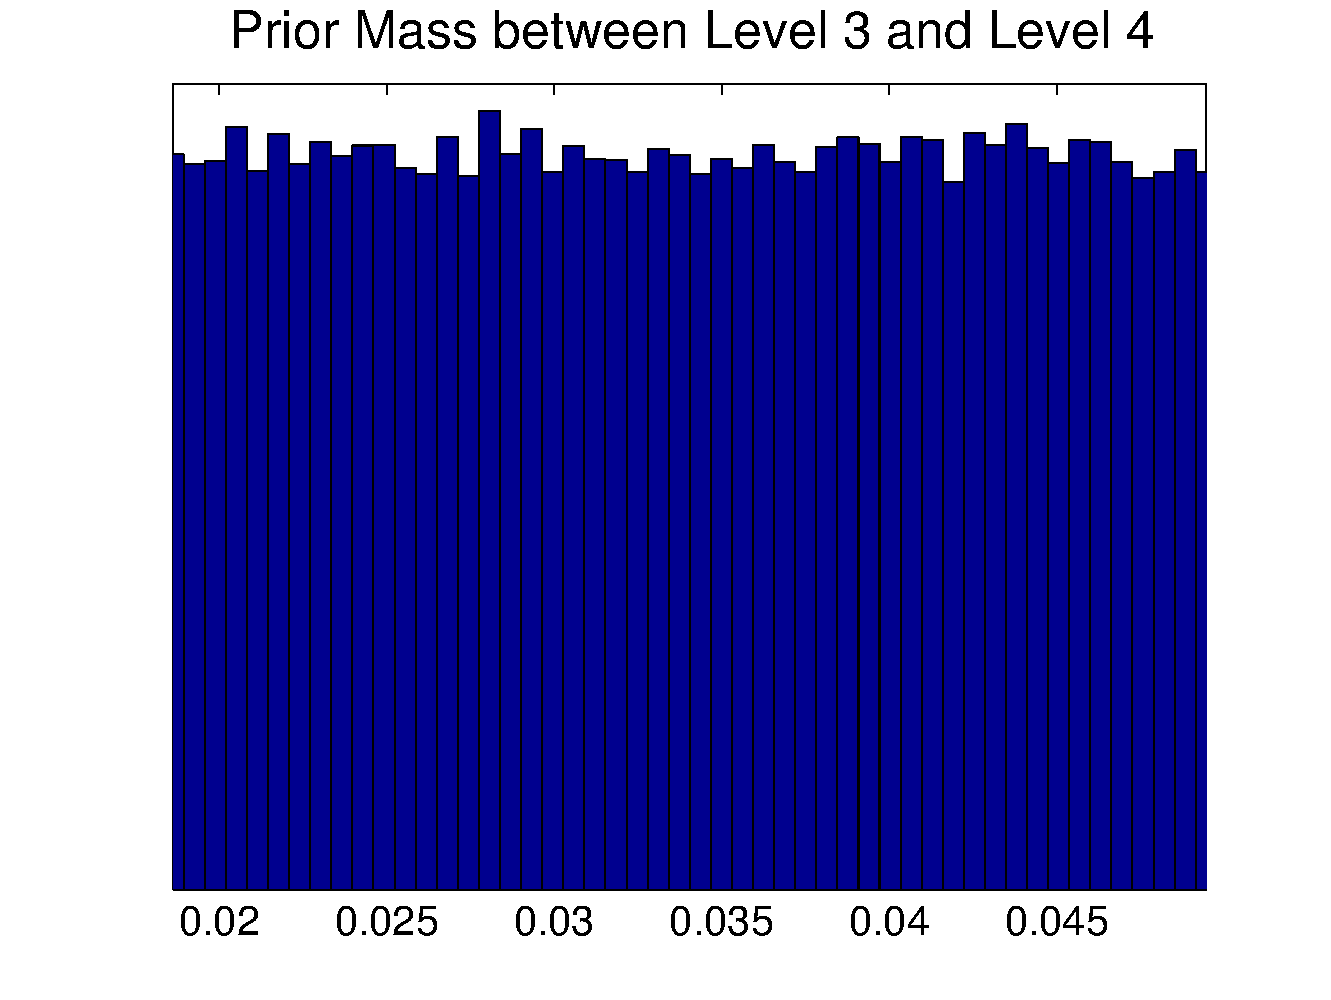
\includegraphics[width=0.45\linewidth]{histgaps-03-04.pdf}\\
 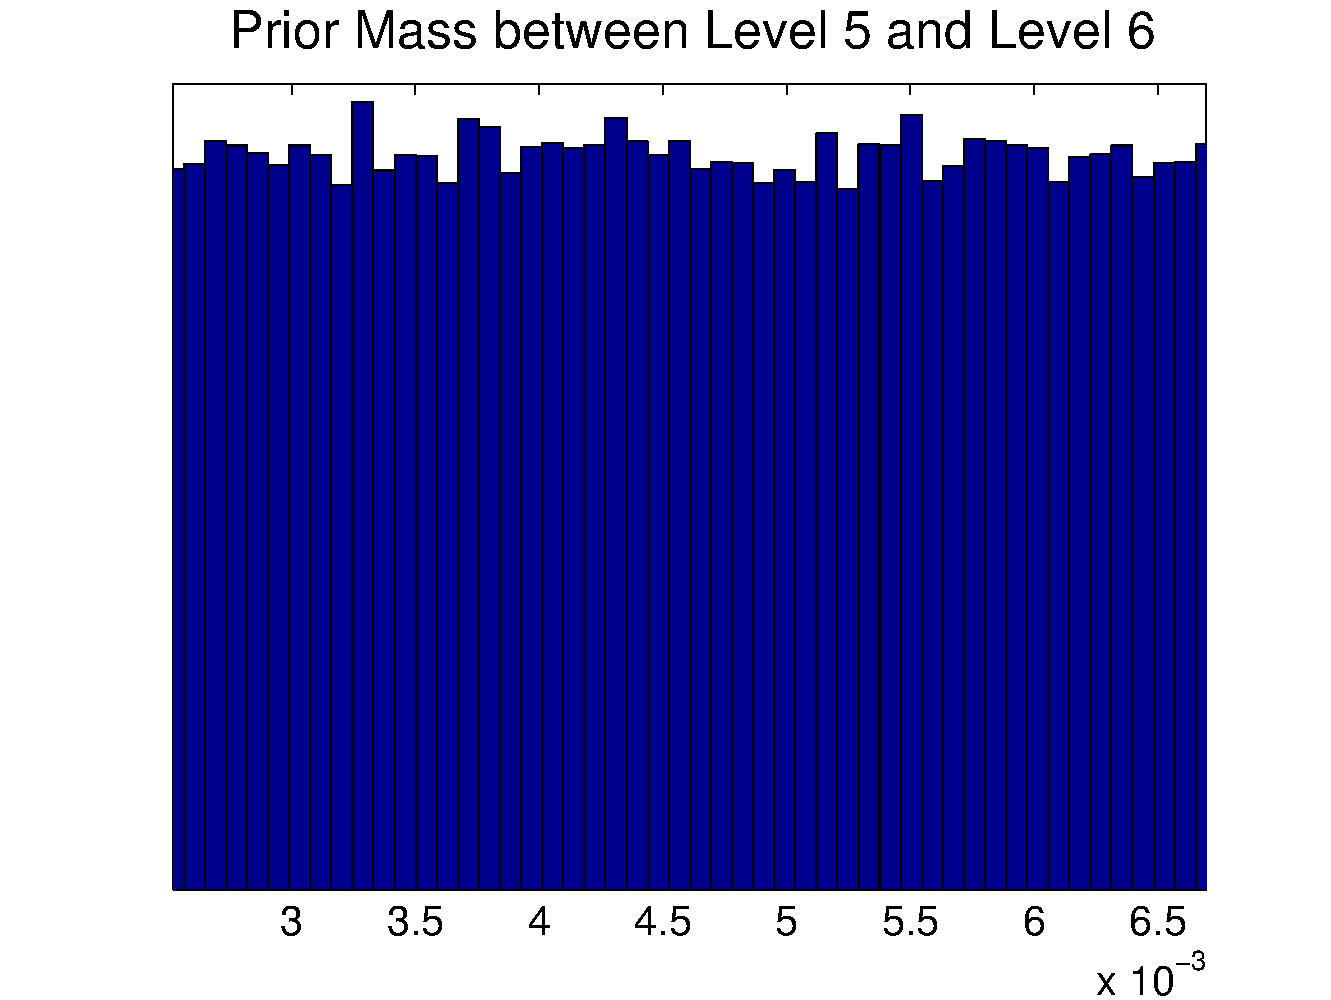
\includegraphics[width=0.45\linewidth]{histgaps-05-06.pdf}
 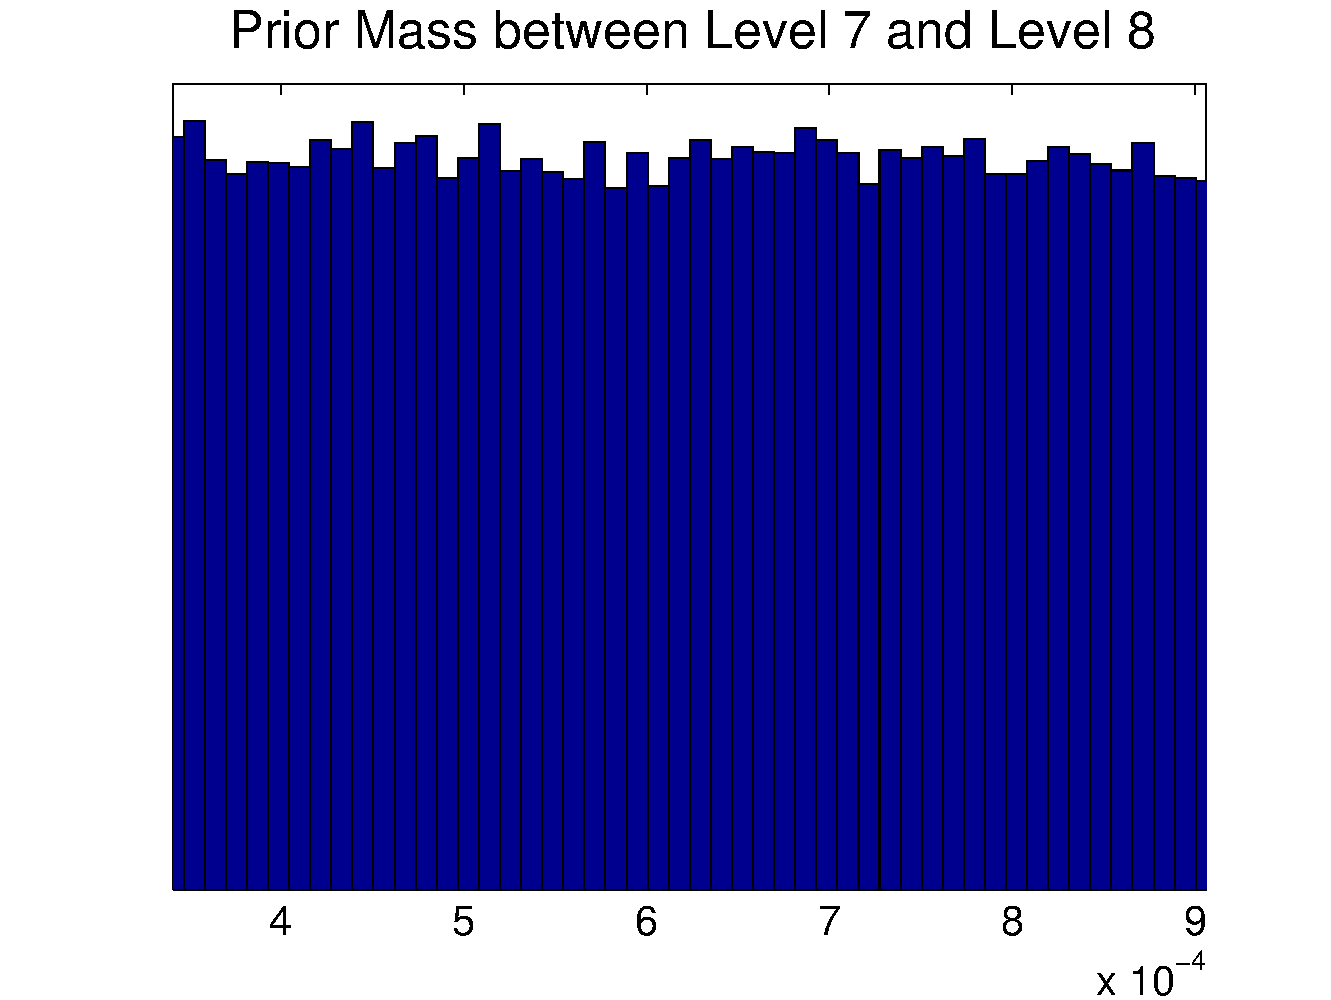
\includegraphics[width=0.45\linewidth]{histgaps-07-08.pdf} \\
\caption{Histograms of prior masses of samples inside a bin sandwiched by two adjacent levels. 4 examples are given. All are approximately uniform distribution.}
 \label{fig:hist-gaps}
\end{figure}

\begin{figure}[h]
 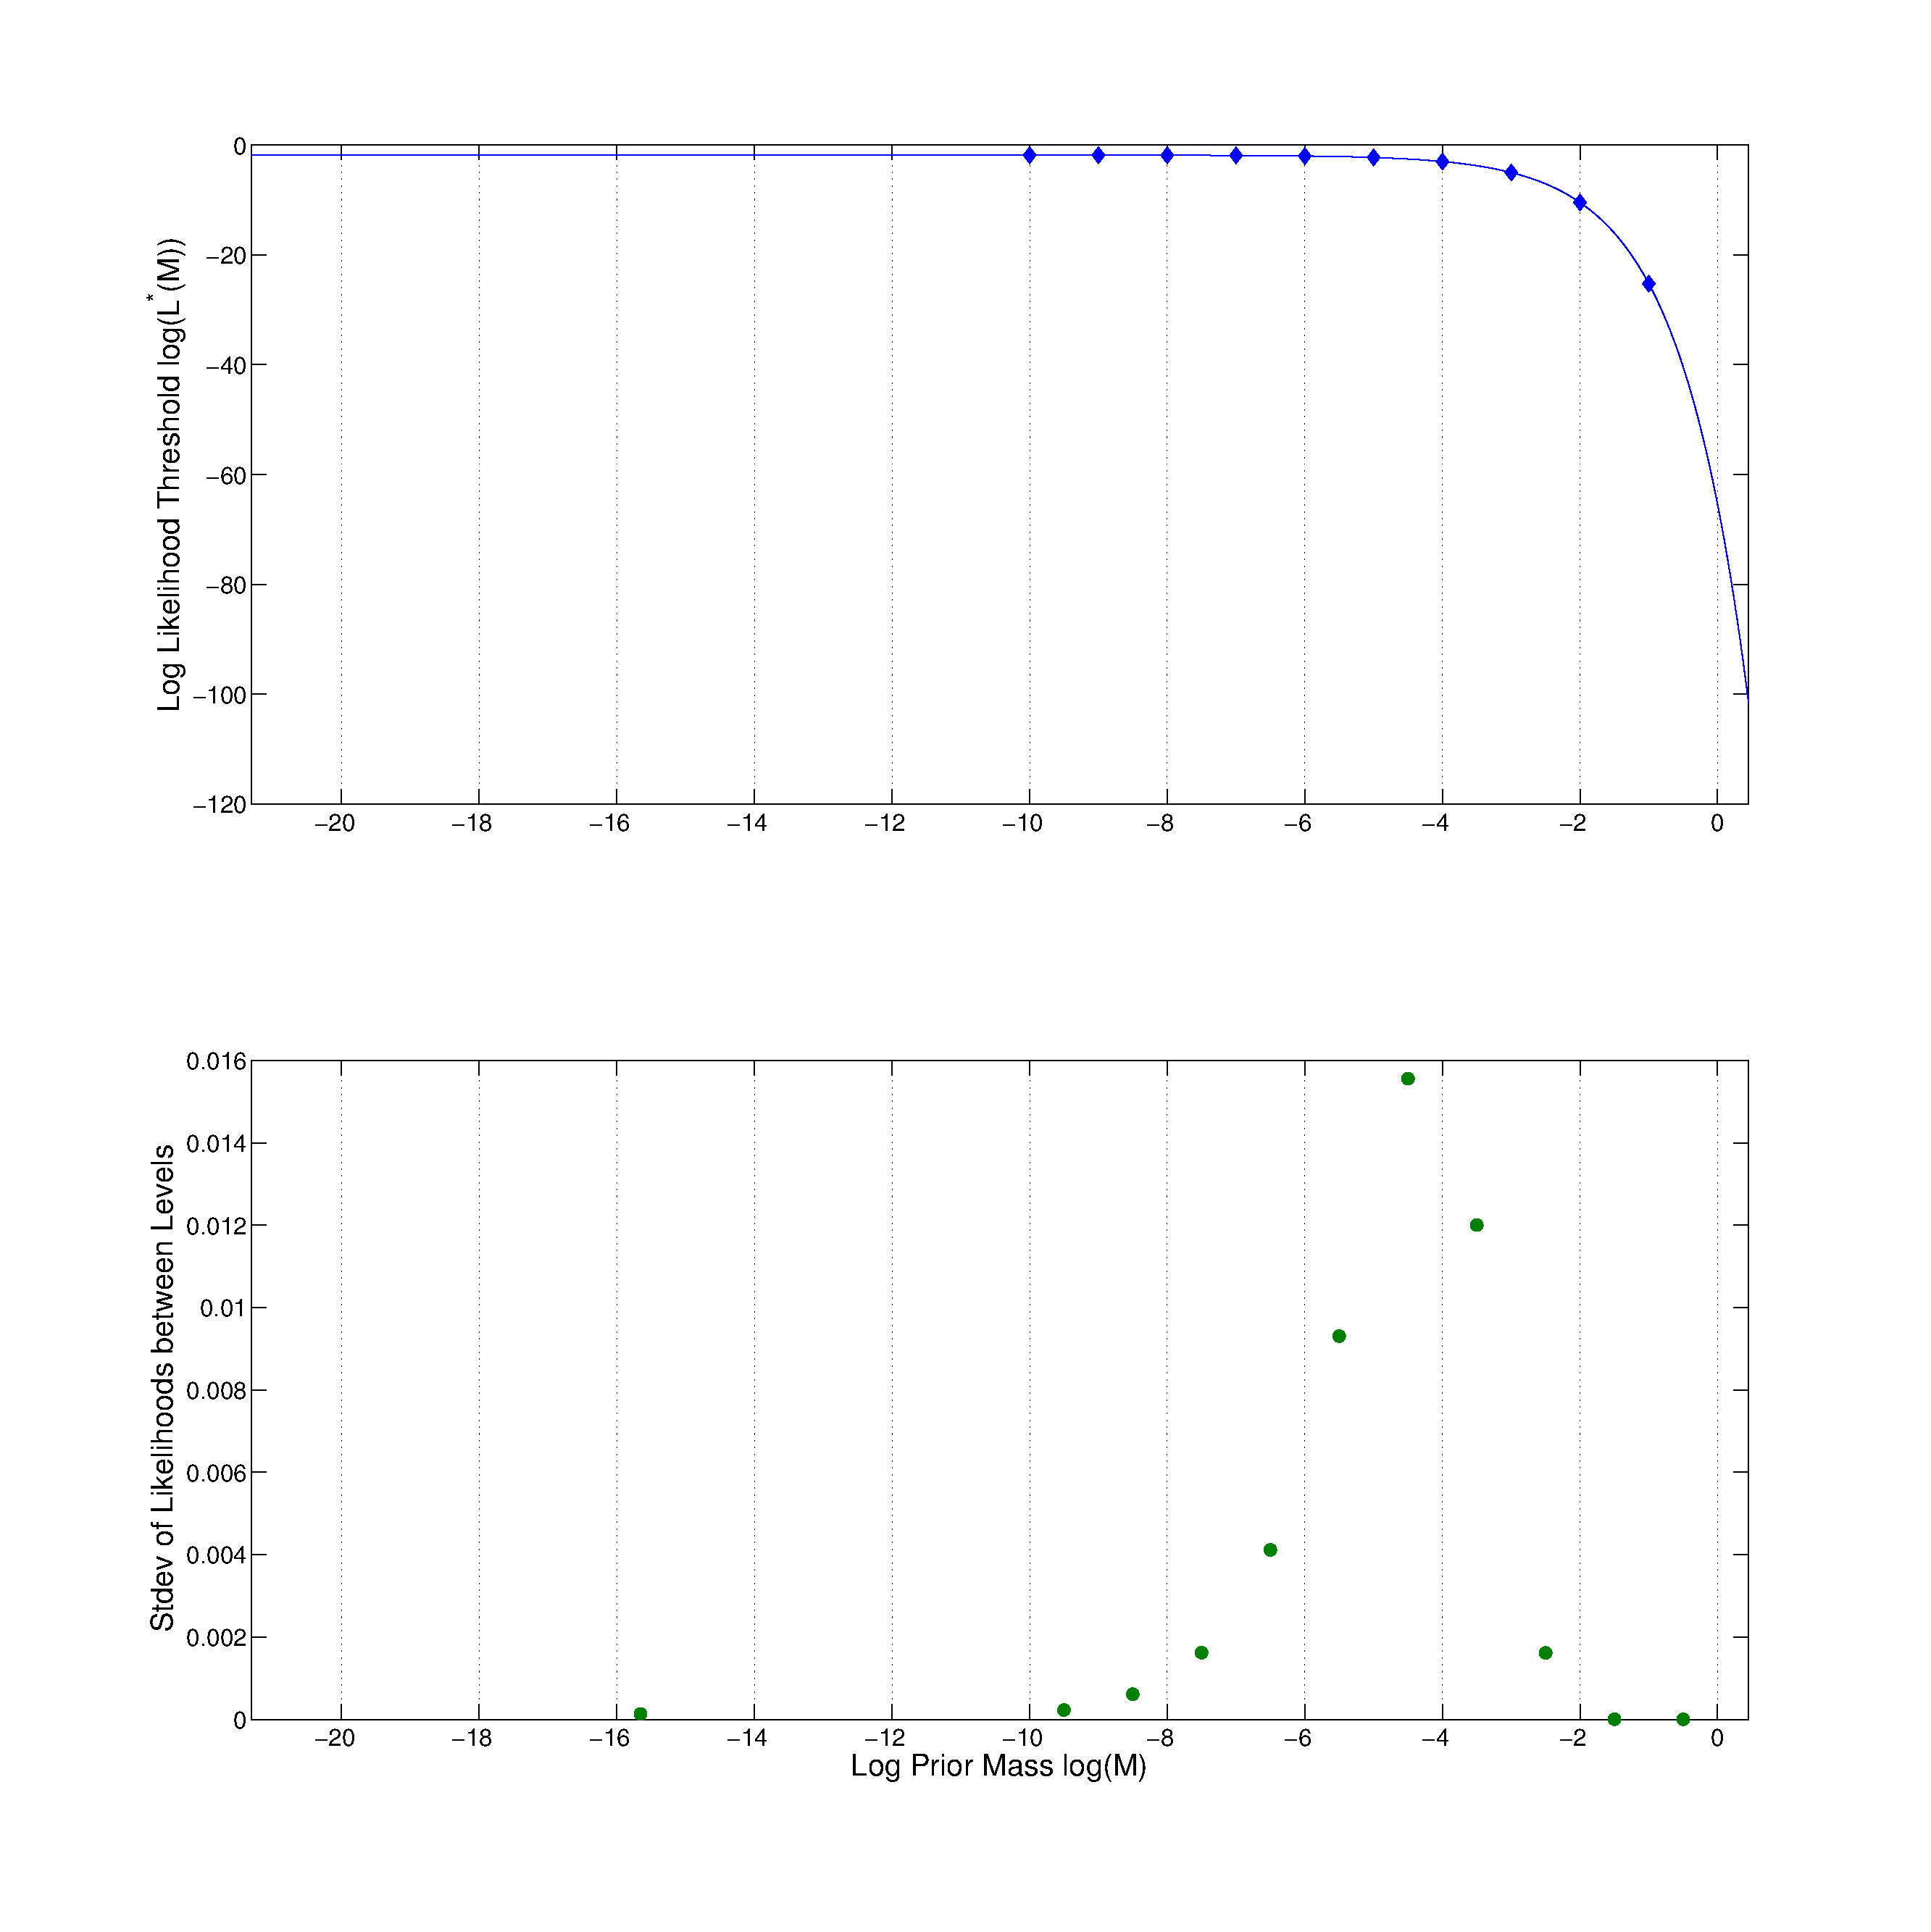
\includegraphics[width=0.99\linewidth]{stdev-between-gaps.pdf}
\caption{The 10 levels in the figure are the true levels summarized in Tab. (\ref{tab:true-levels}). Notice that the standard deviation of likelihood samples between level 3 ($\log{M} = -3$) and level 6 ($\log{M} = -6$) will pretty much determine the standard deviation of the final result.}
 \label{fig:level-var}
\end{figure}

\begin{table}[h]
\centering
std for 10-d case ($\times10^{-15}$)\\
\begin{tabular}{c|c|c|c}
\hline
 & $N_1=10^4$ & $N_1=3\times10^4$ & $N_1=10^5$\\
\hline
$N_2=10^6$                  & 3.1760  & 3.2465 & 3.1653 \\
$N_2=3\times10^6$ & 1.8297  & 1.8816 & 1.8390 \\
$N_2=10^7$                  & 0.9887  & 0.9704 &  1.0238\\
\hline
\end{tabular}
\caption{The standard deviations for different $N_1$'s and $N_2$'s. The experiments are repeated for $1,000$ times. Compared with evidence value $9.77\times10^{-14}$, all the standard deviations are reasonably small. But $N_2$ is clearly more important in reducing variance. Note that there are 30 levels in this case, $30\times N_1$ and $N_2$ are actually comparable.}
\label{tab:N1N2}
\end{table} 

\begin{figure}
 \centering
 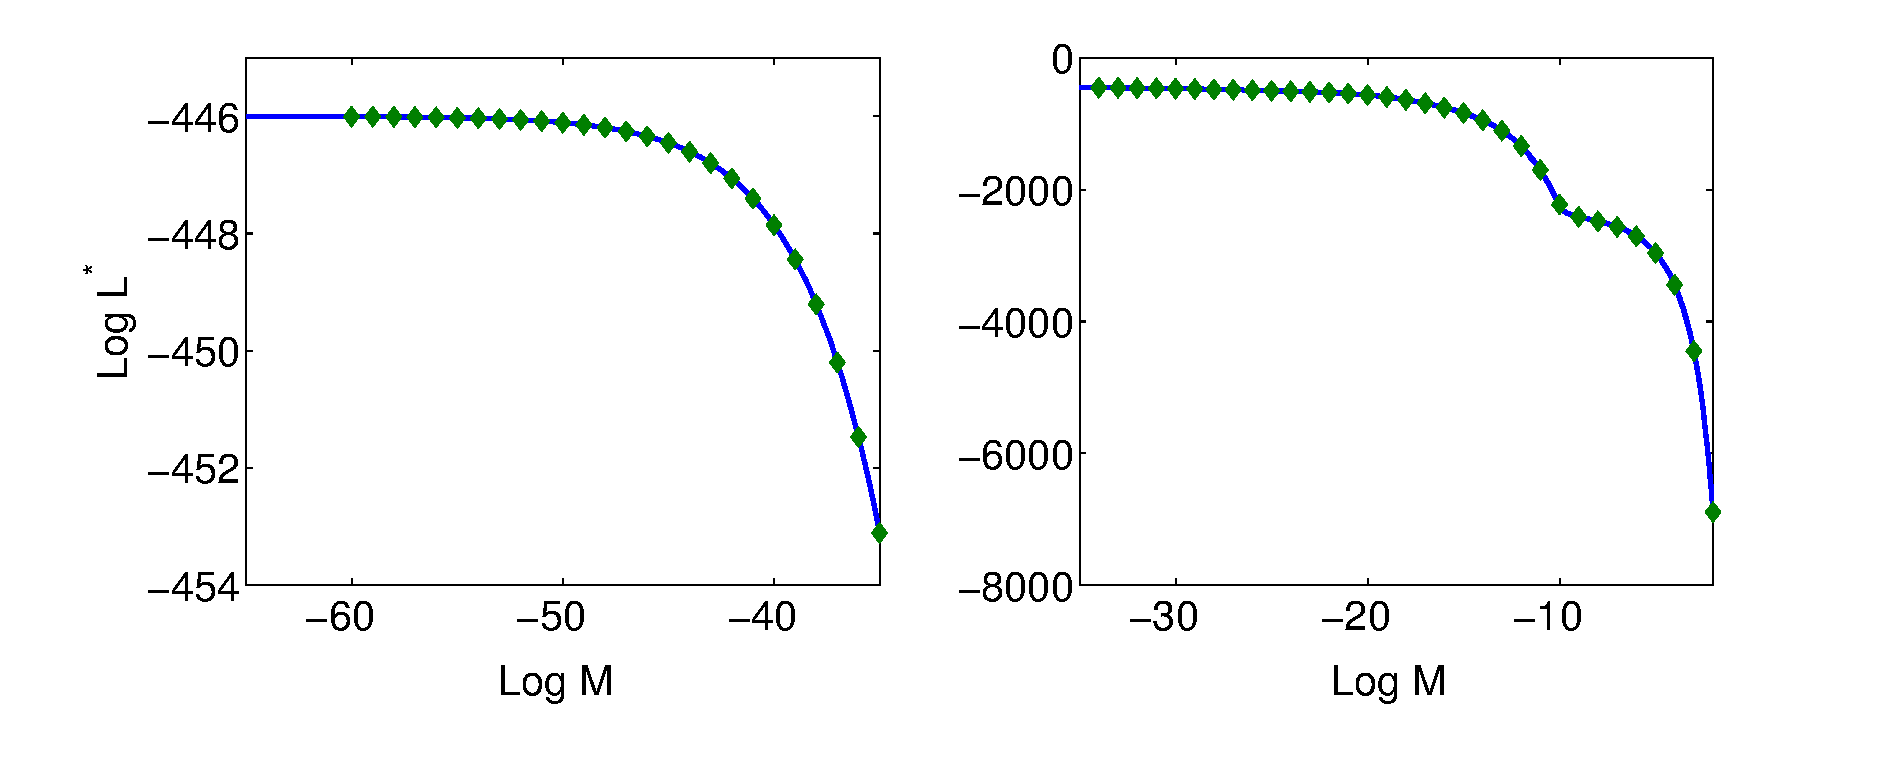
\includegraphics[width=0.99\linewidth]{Level_122_mod_1.pdf}\\
 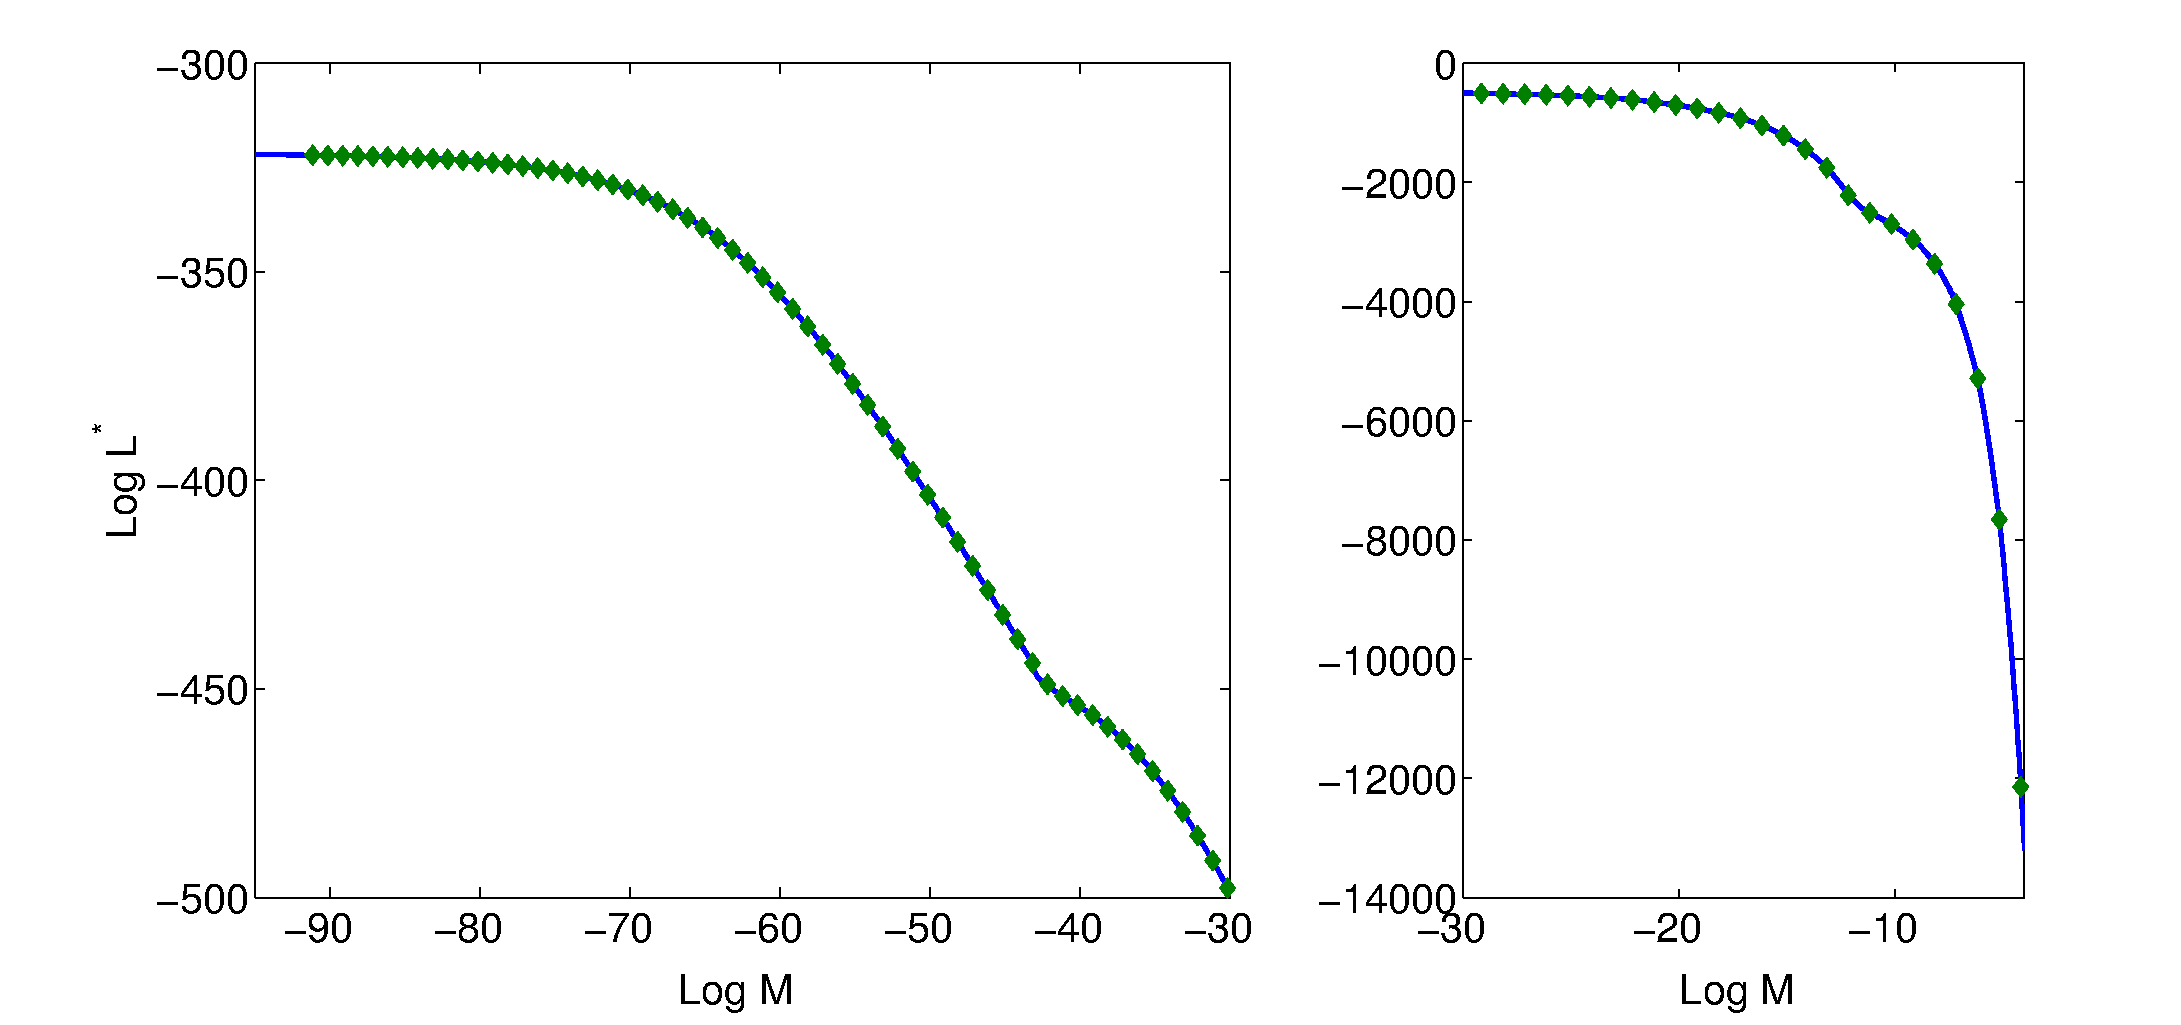
\includegraphics[width=0.9\linewidth]{Level_122_mod_2.pdf}\\
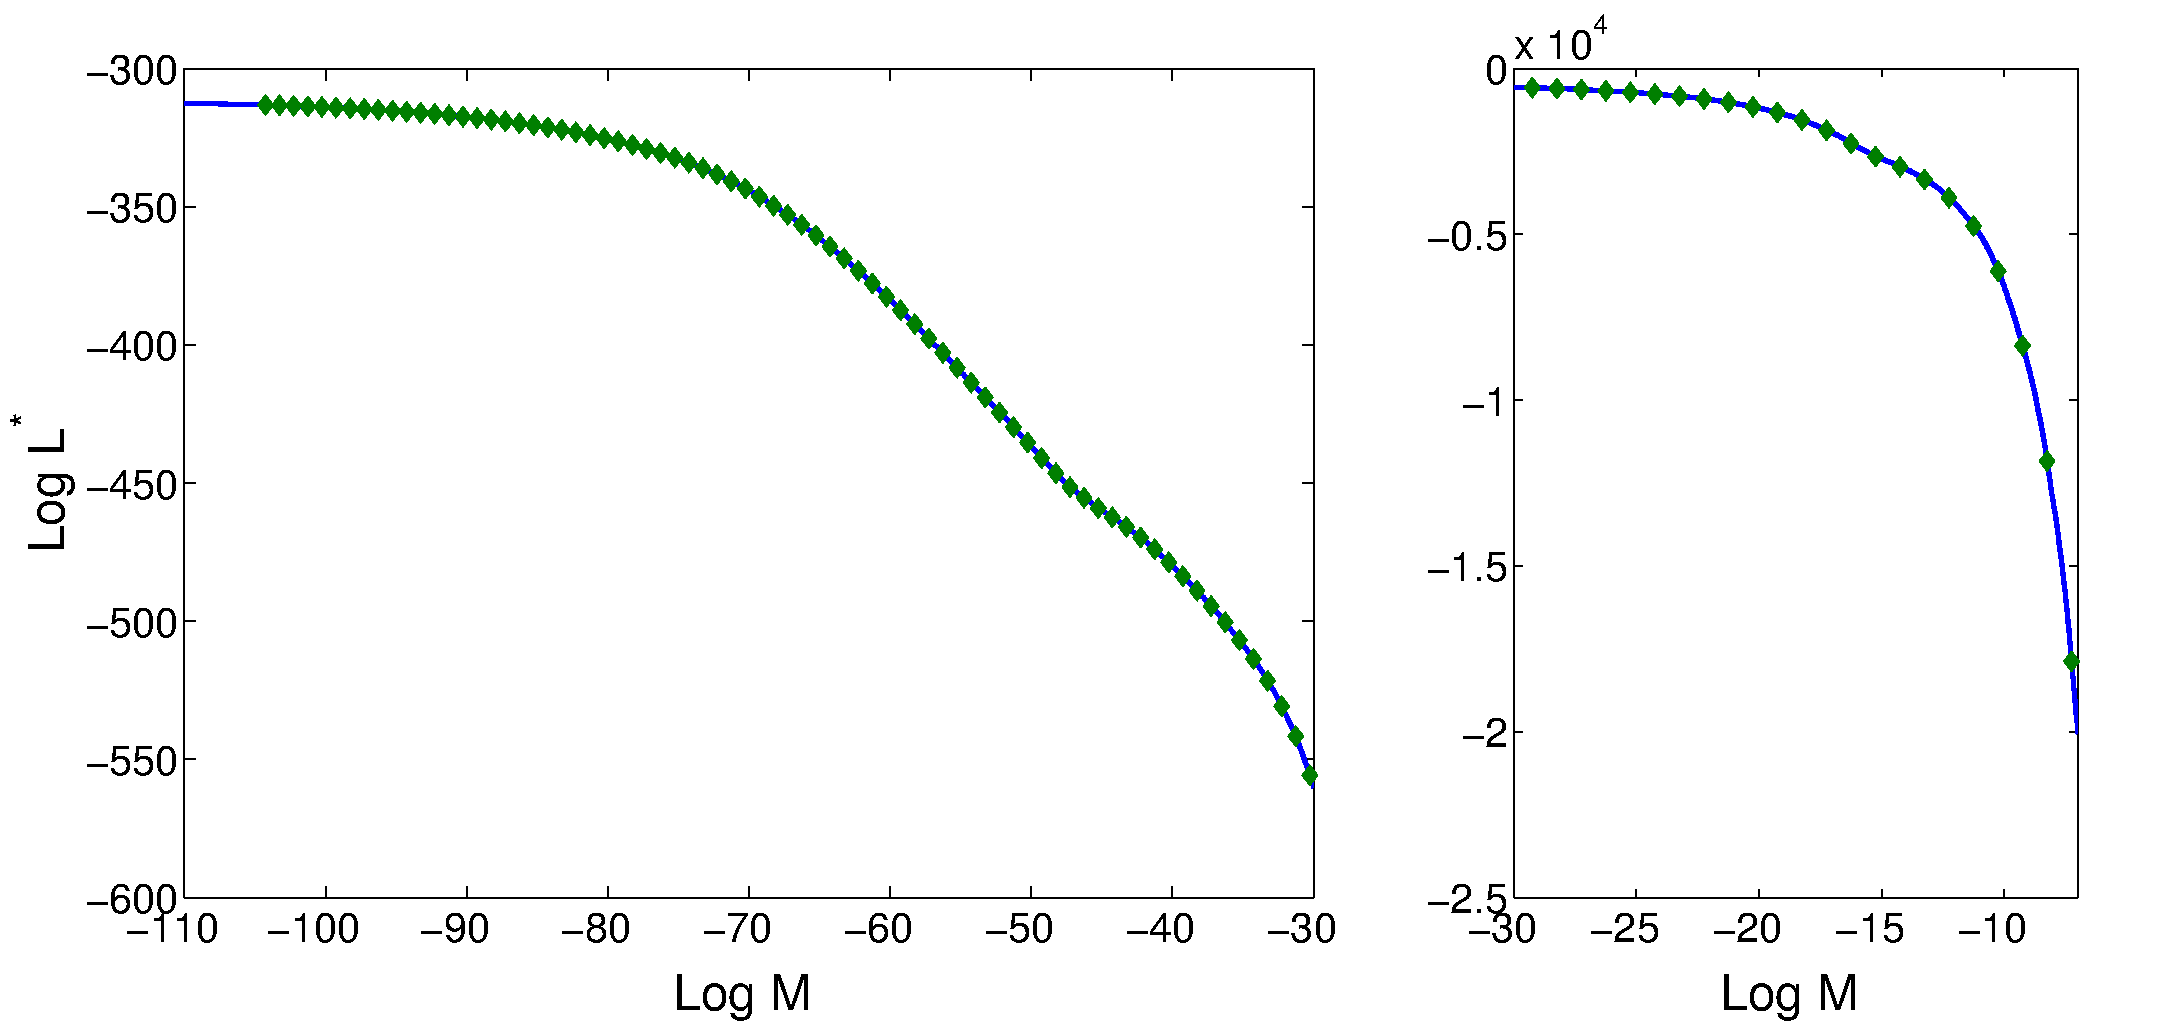
\includegraphics[width=0.9\linewidth]{Level_122_mod_3.pdf}
\caption{The 1st row shows the levels of 1-companion model. The 2nd row shows the levels of 2-companion model. The 3rd row shows the levels of 3-companion model.}
 \label{fig:levels-122}
\end{figure}

\begin{figure}
 \centering
 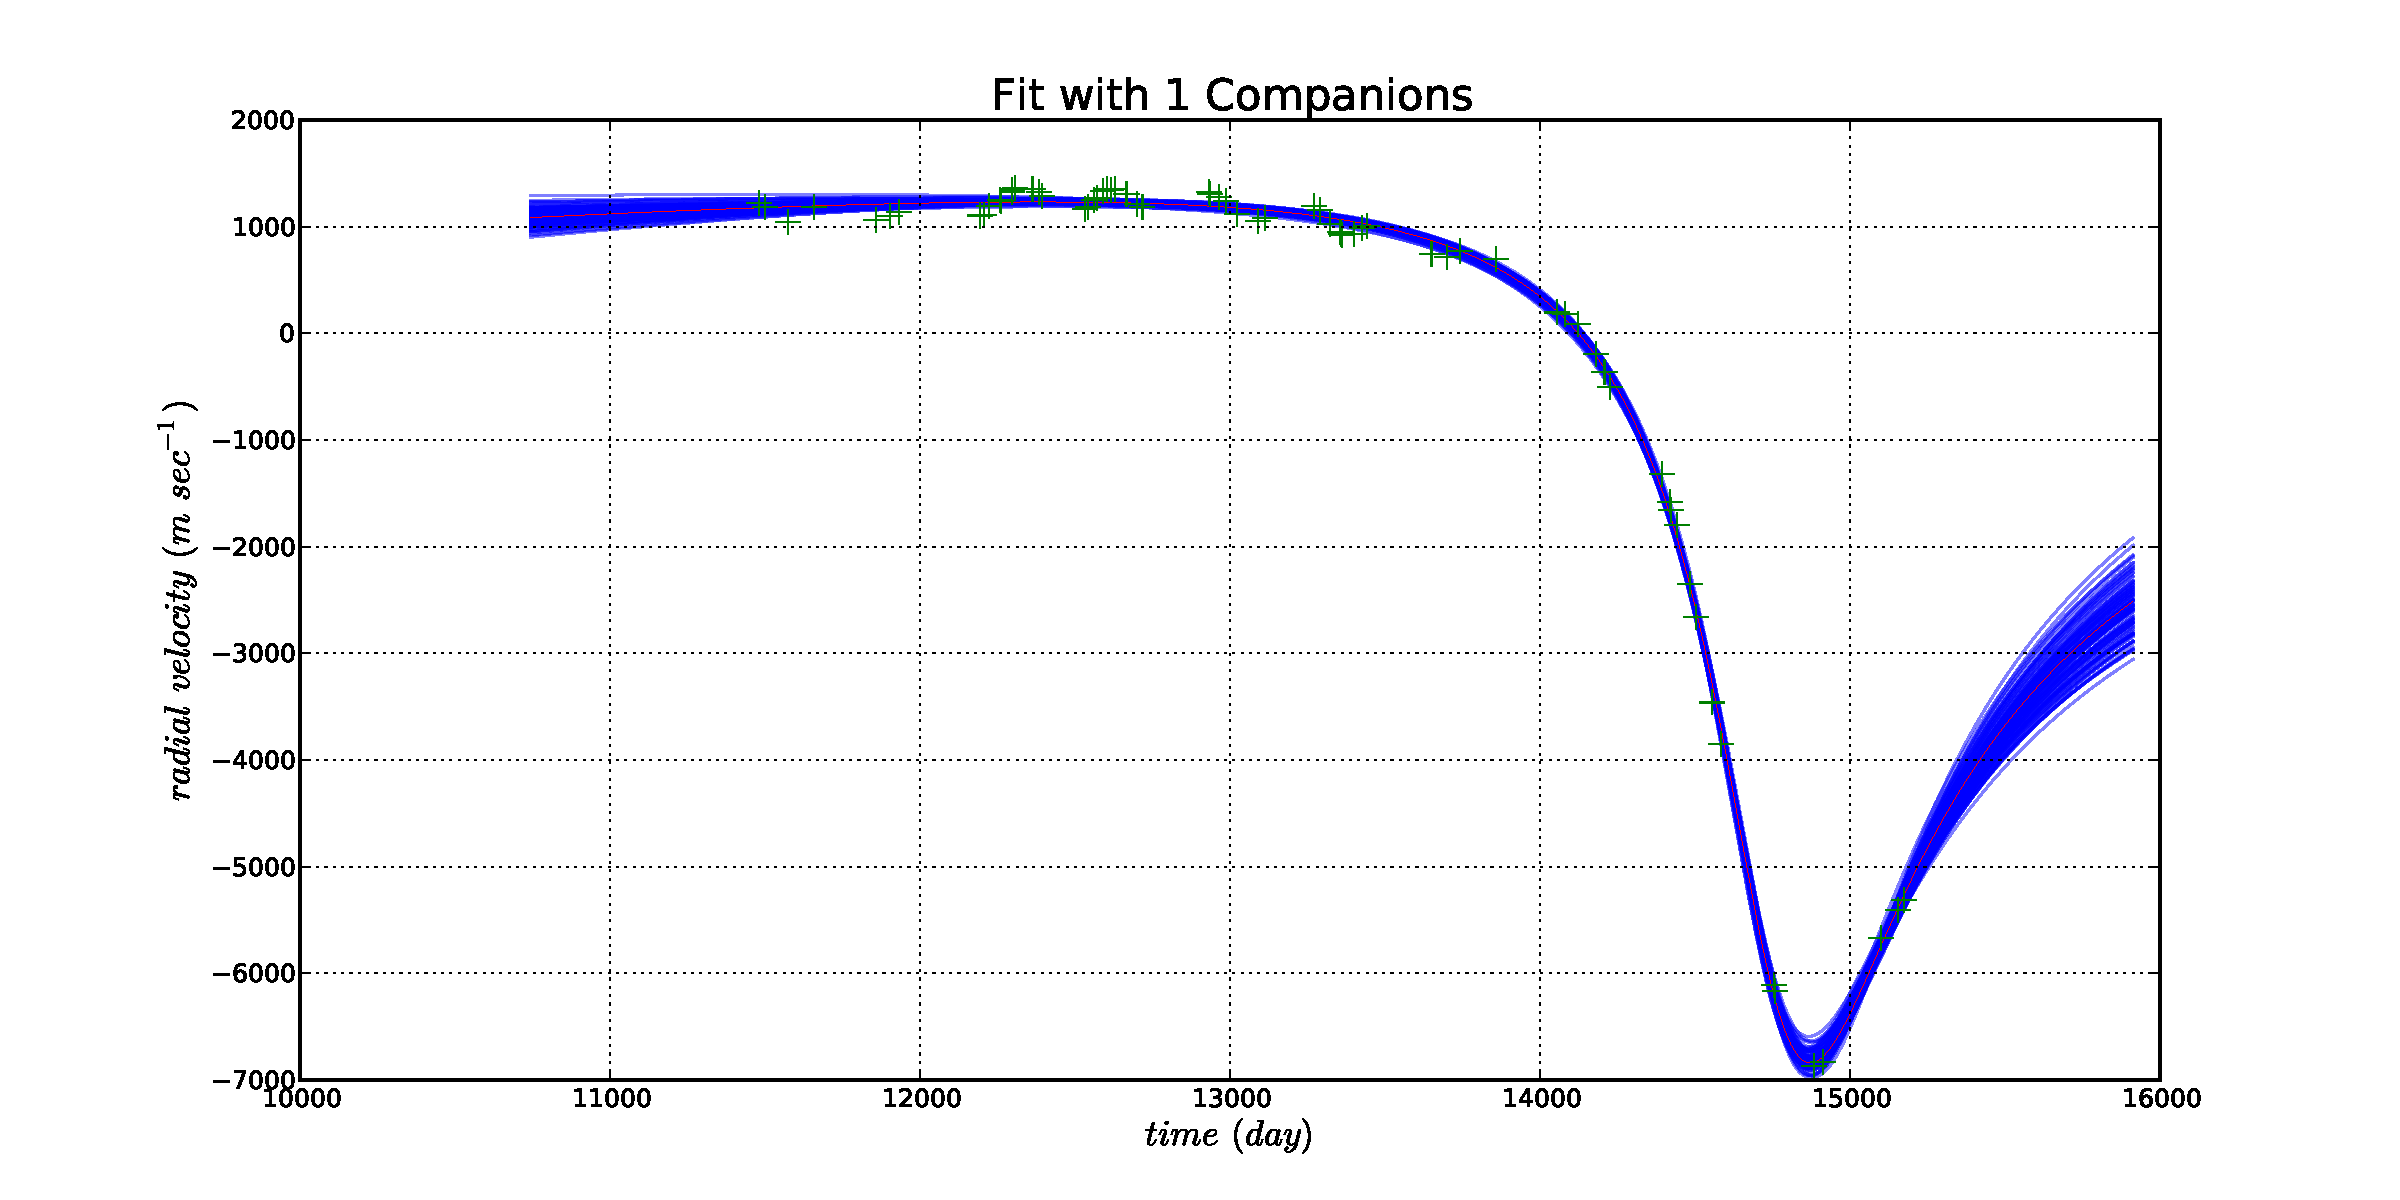
\includegraphics[width=0.85\linewidth]{fit_122_comp_1.pdf}\\
 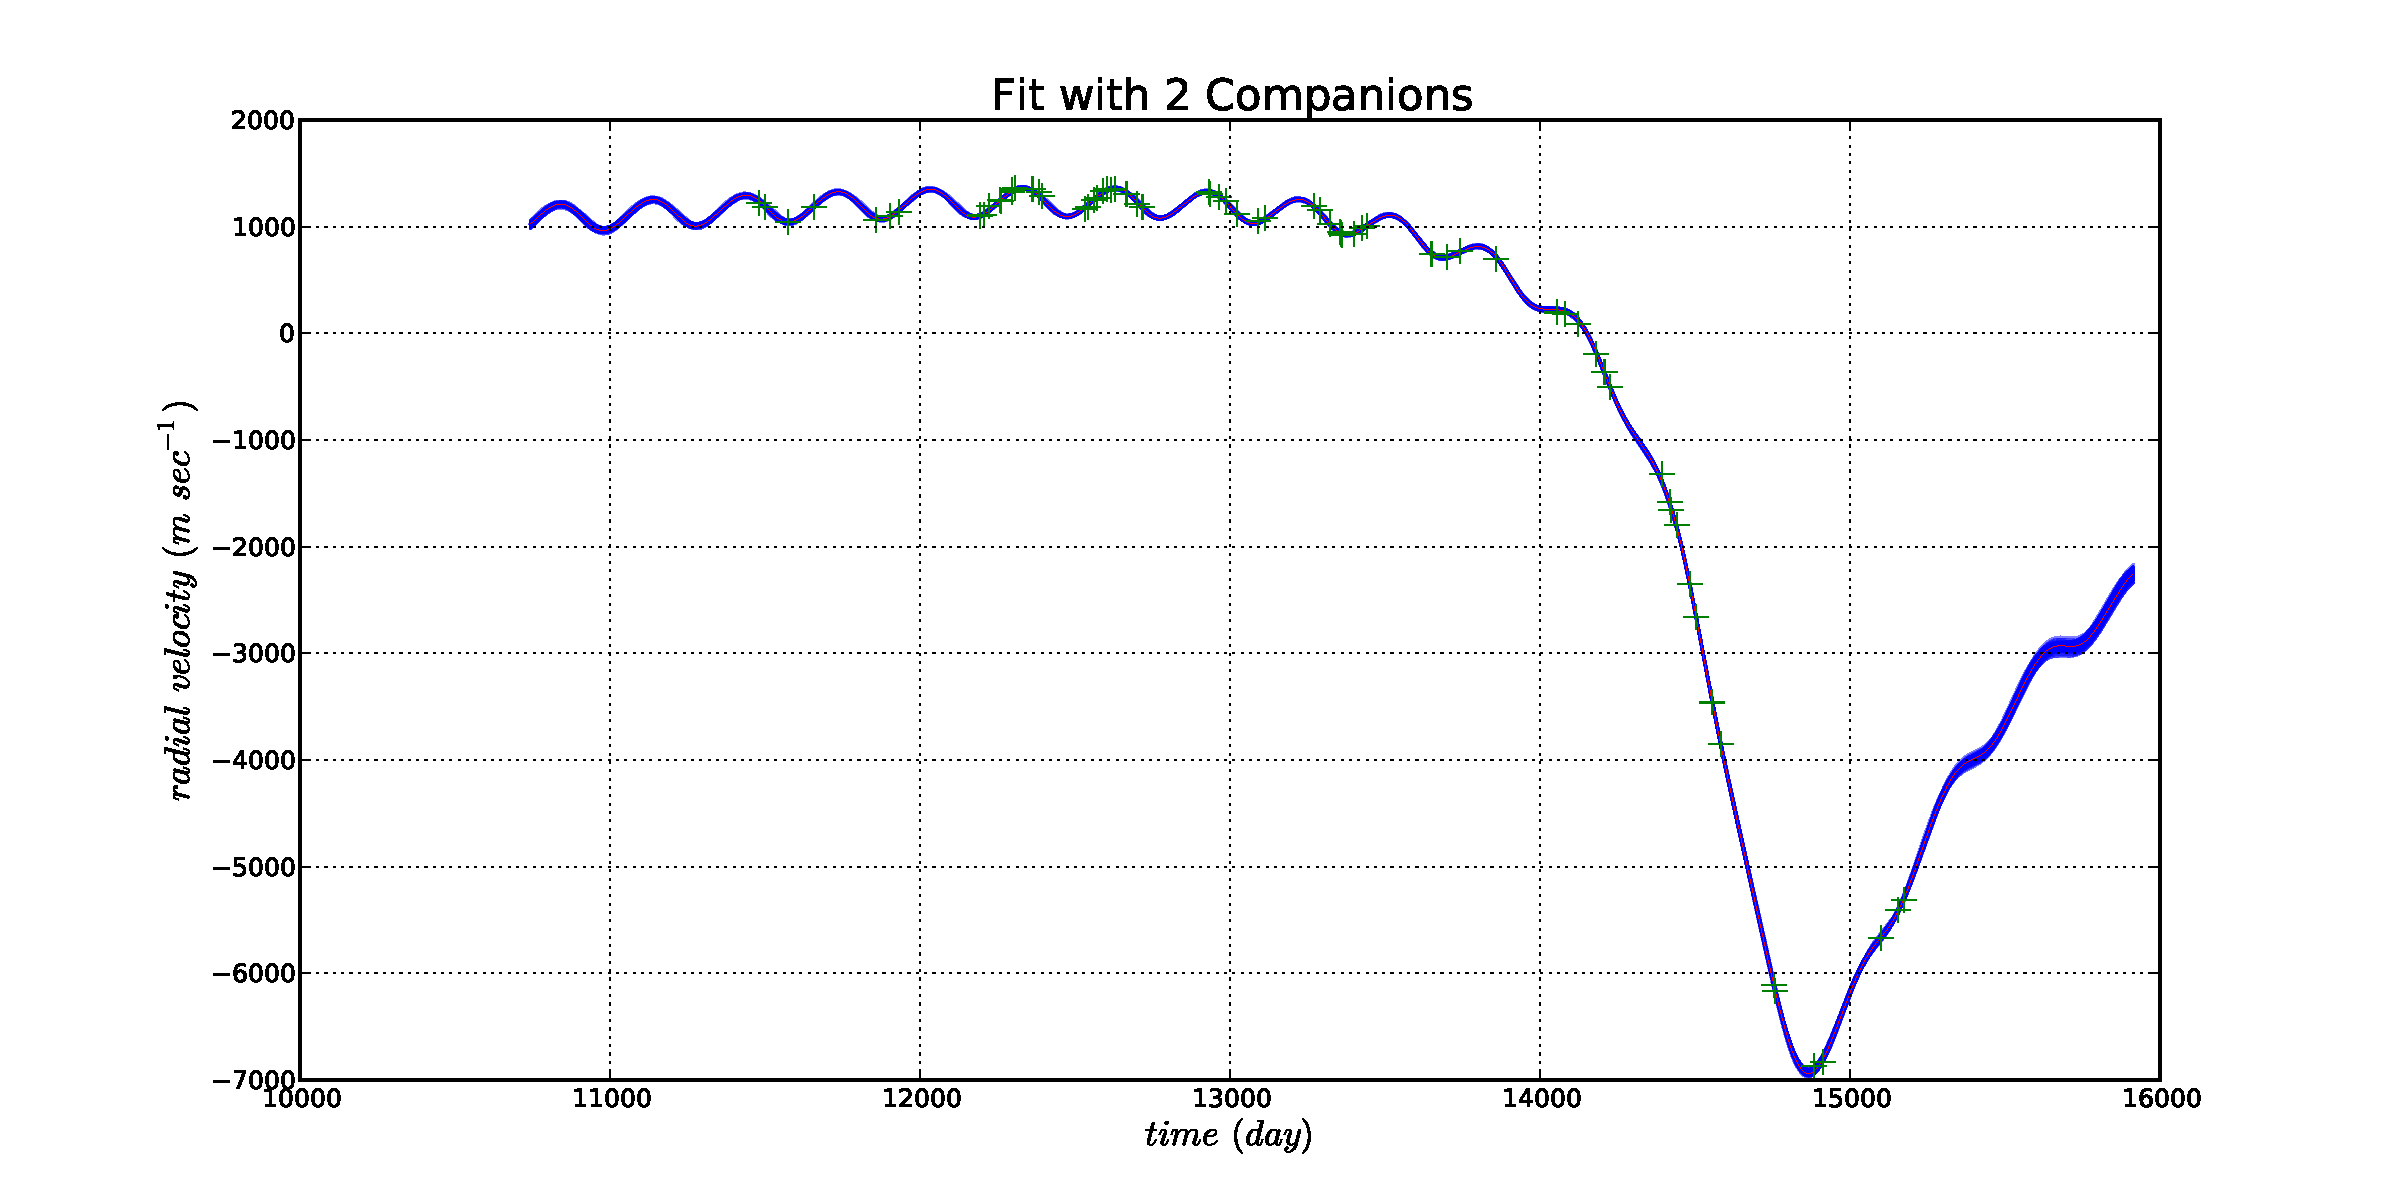
\includegraphics[width=0.85\linewidth]{fit_122_comp_2.pdf}\\
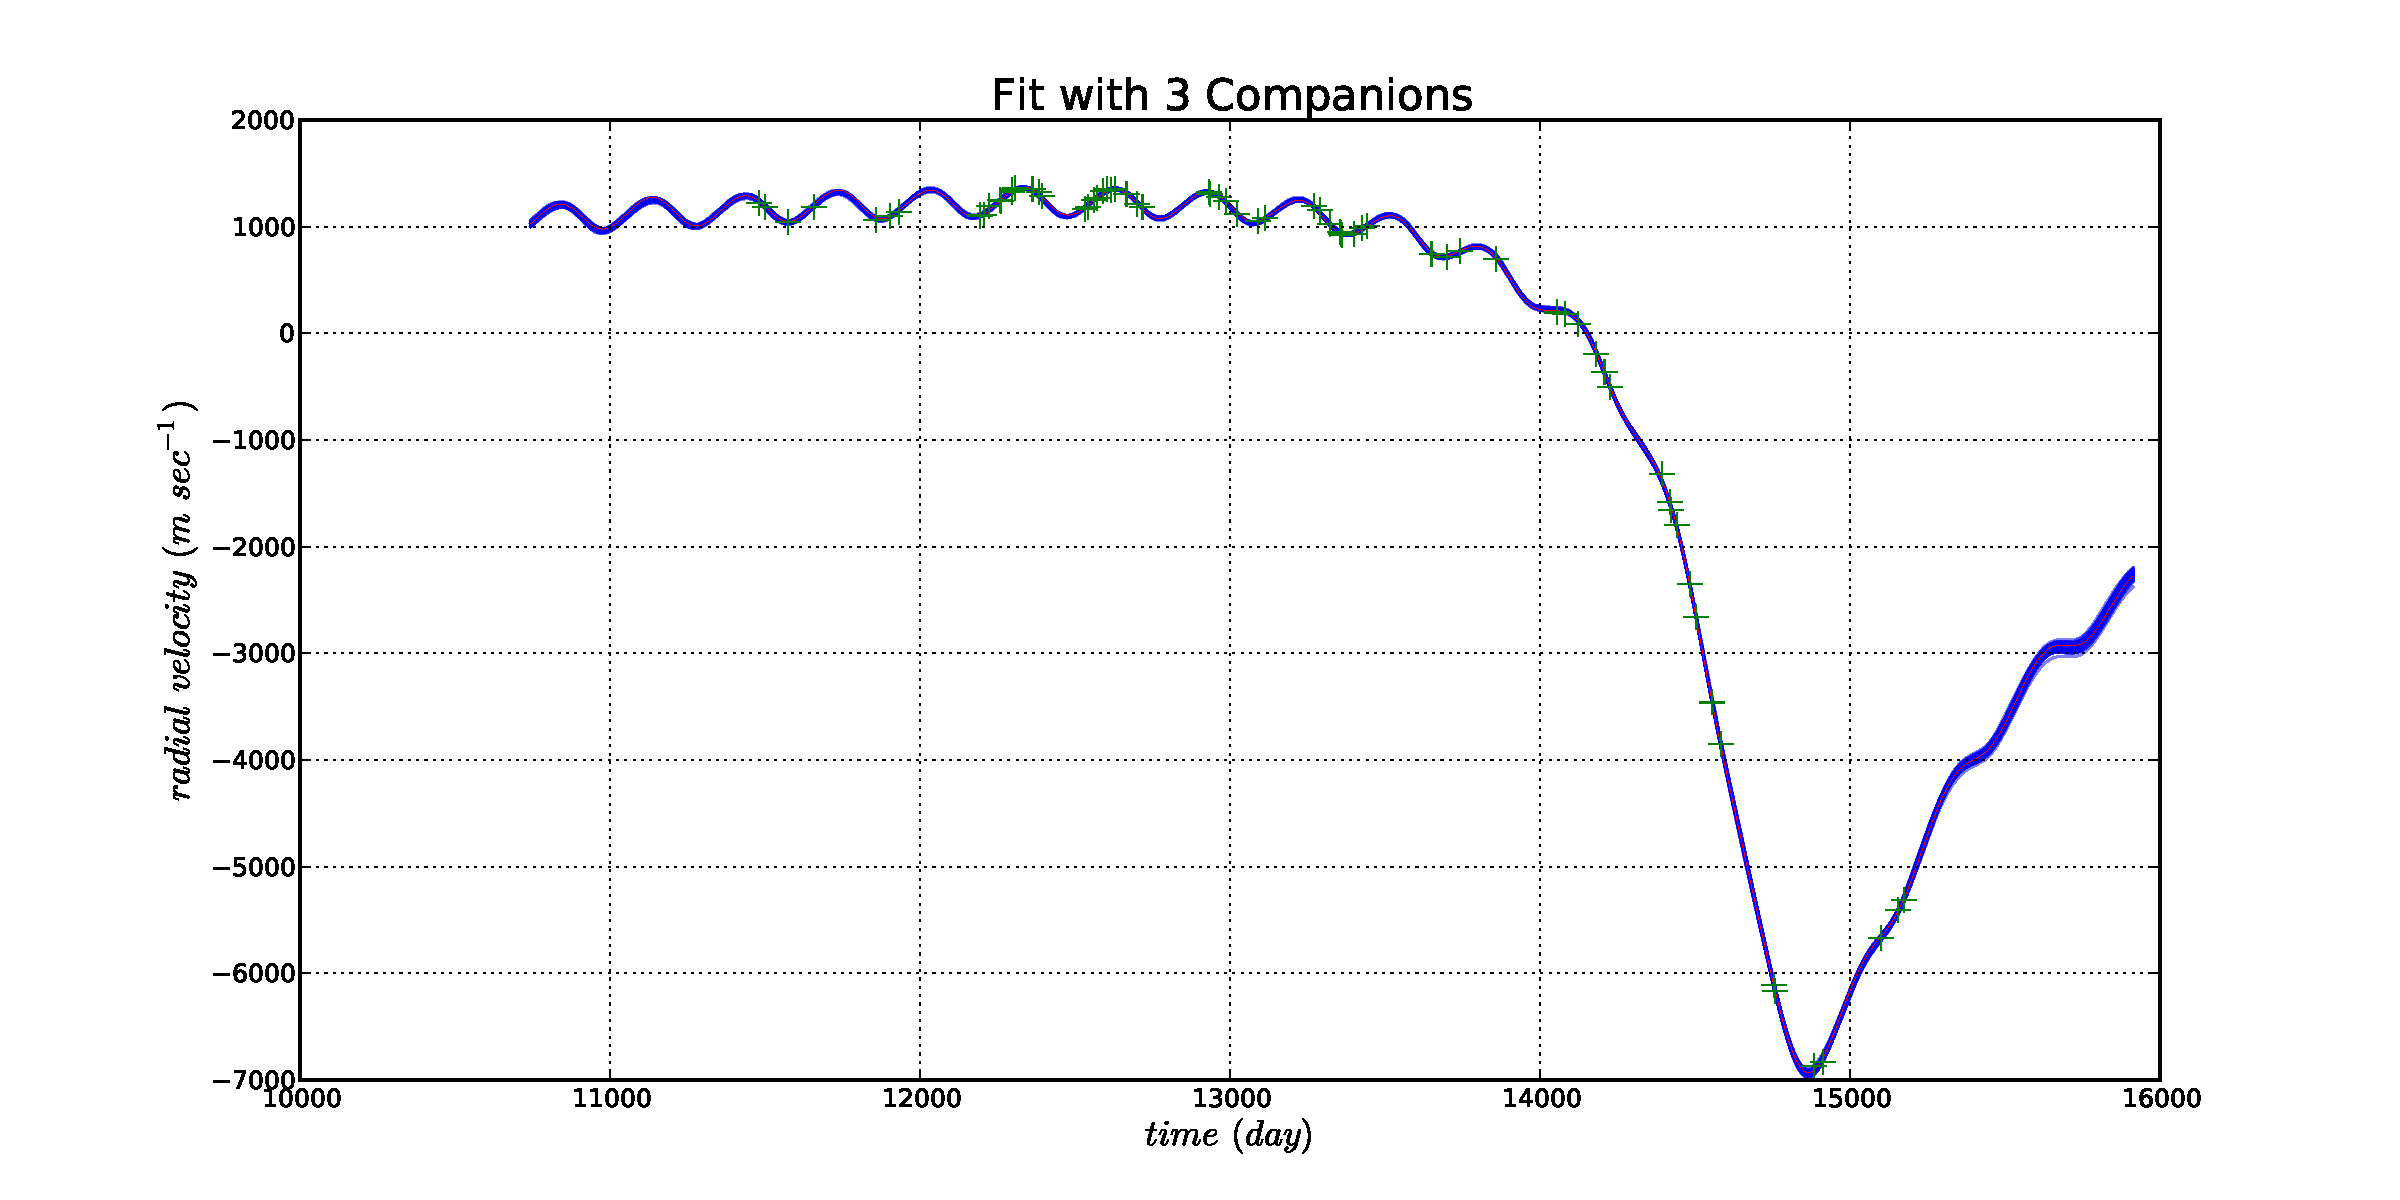
\includegraphics[width=0.85\linewidth]{fit_122_comp_3.pdf}
\caption{The 1st row shows the fit of 1-companion model. The 2nd row shows the fit of 2-companion model. The 3rd row shows the fit of 3-companion model. All the fits are drawn from the posterior of each model. The companion model is clearly not as good as the other two. The 2-companion and 3-companion models are not distinguishable from this view.}
 \label{fig:fit-122-1-2-3}
\end{figure}

\begin{figure}
 \centering
 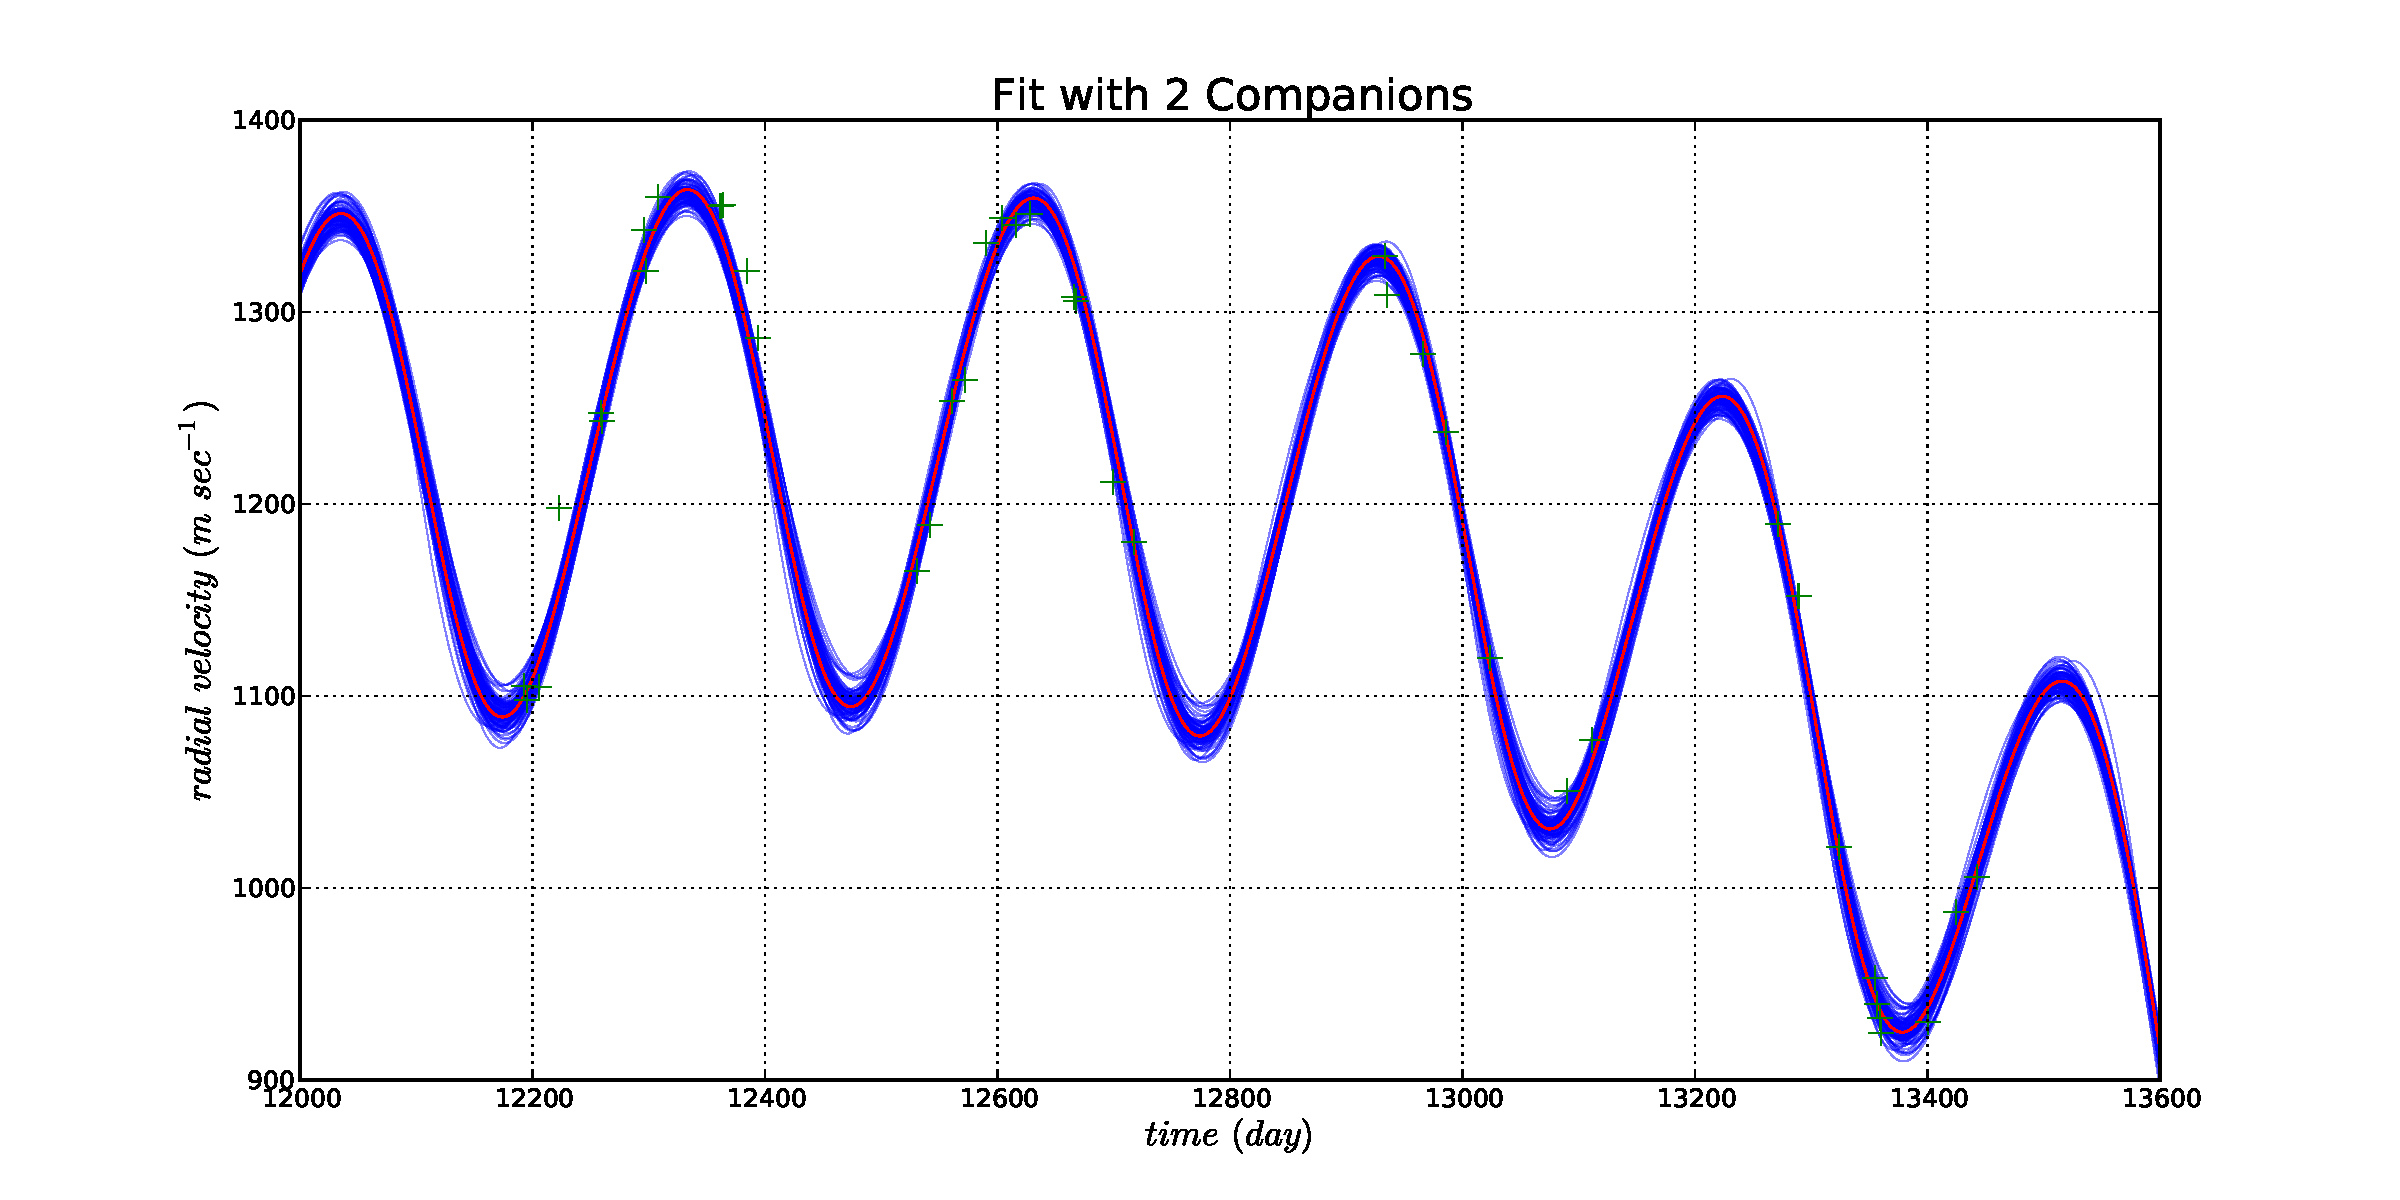
\includegraphics[width=0.99\linewidth]{fit_122_comp_2_small.pdf}\\
 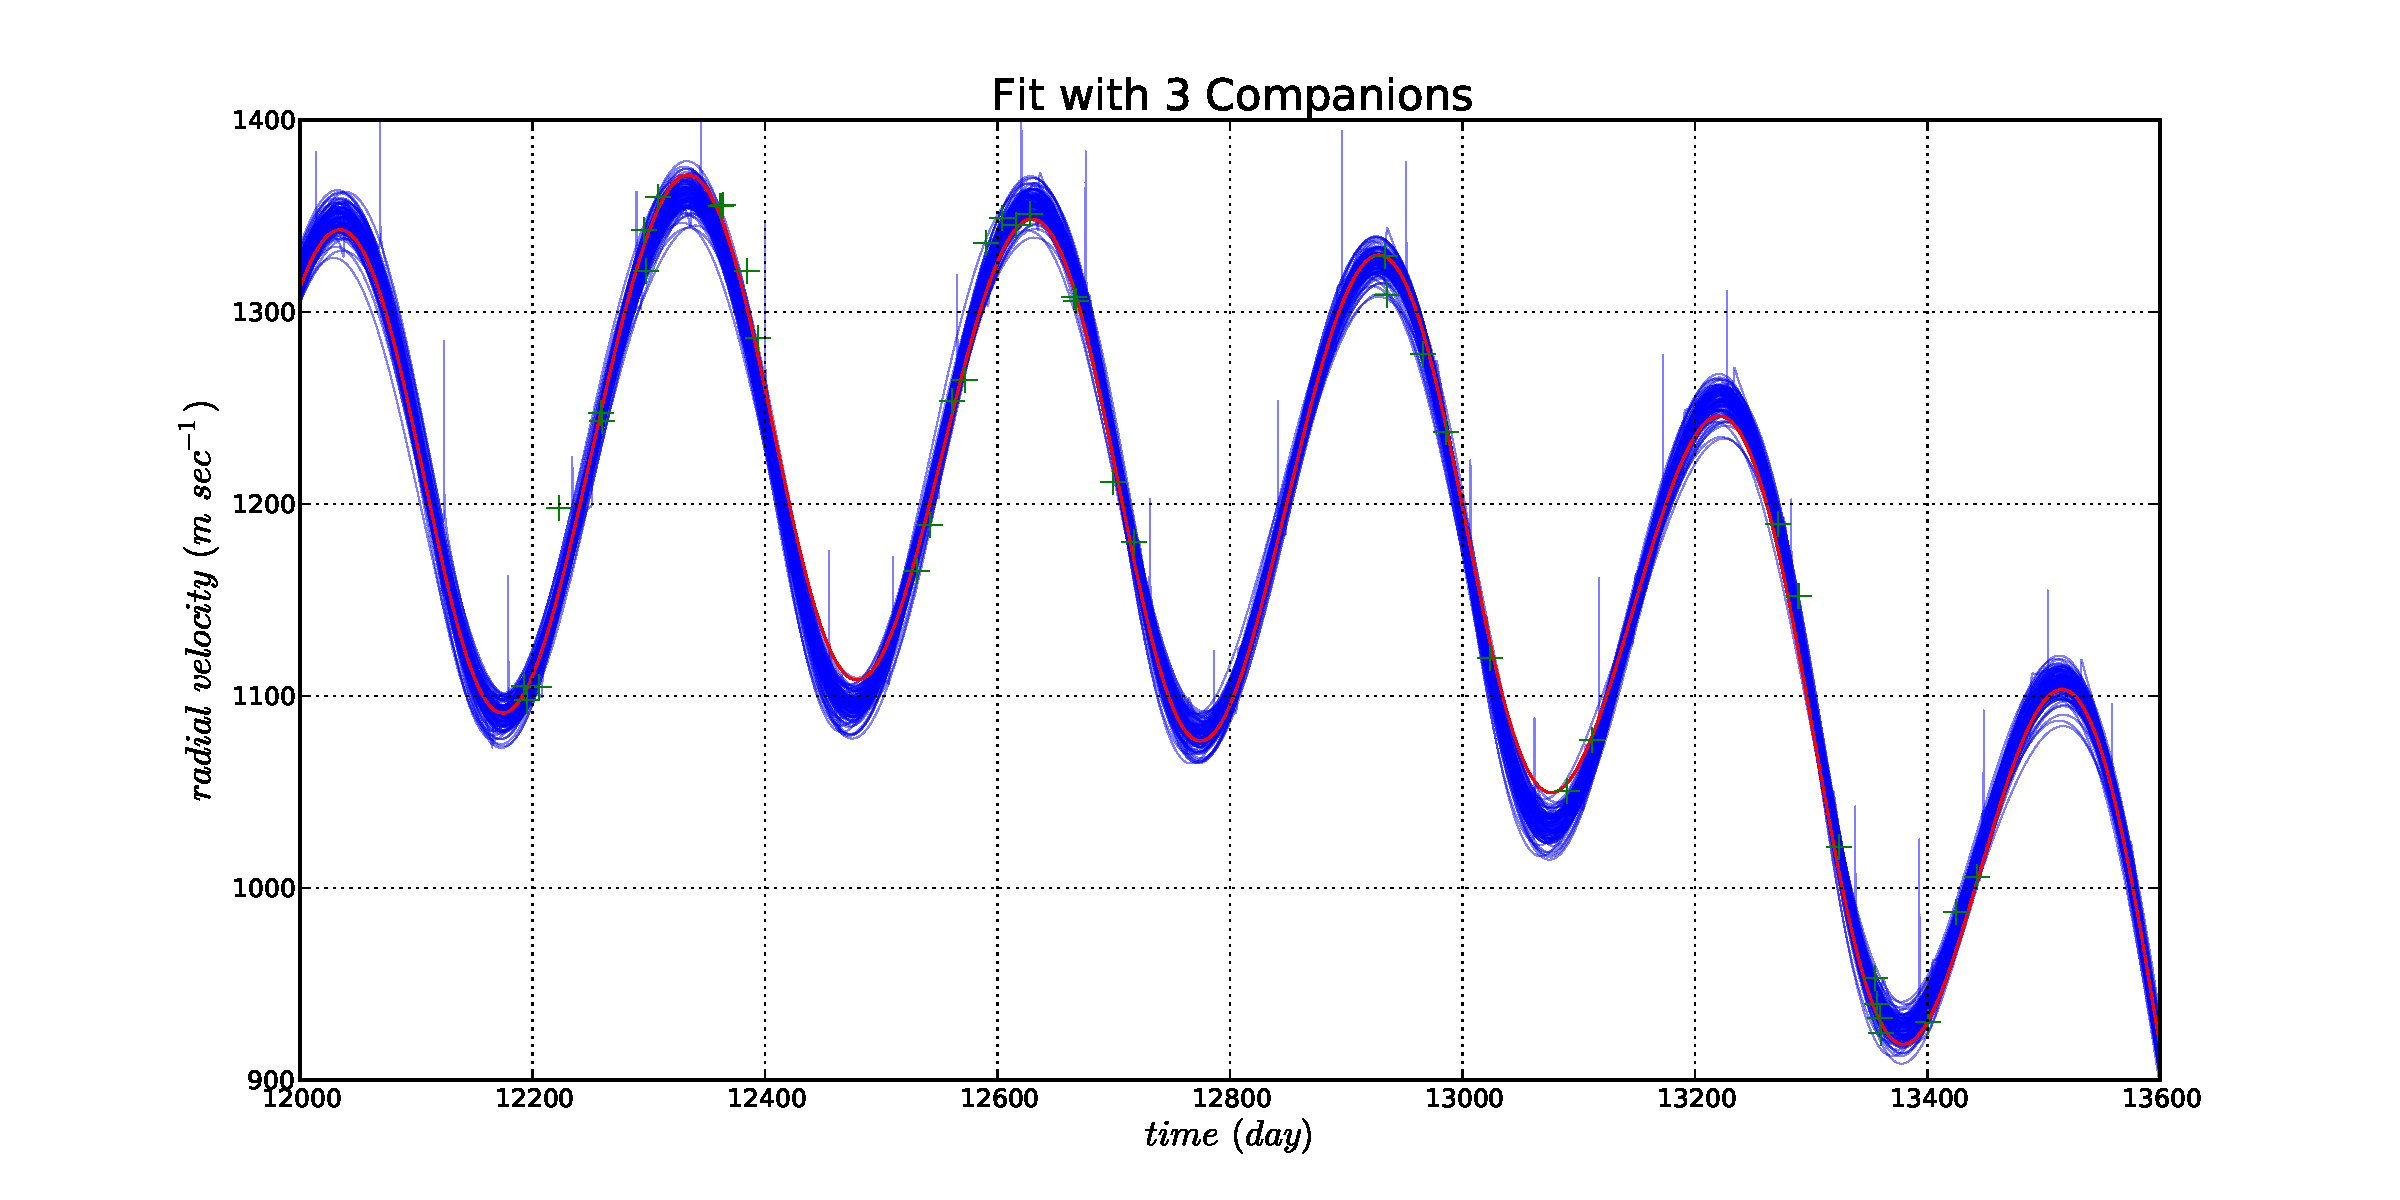
\includegraphics[width=0.99\linewidth]{fit_122_comp_3_small.pdf}
\caption{The 1st row shows the fit of 2-companion model zoomed in.  The 2nd row shows the fit of 3-companion model zoomed in. The \textcolor{red}{red curves} in the center indicate the optimal fits. The 3-companion fit is only slightly better than the 2-companion fit. Because the optimally-fit 'well' in the 3-companion fit is too shallow. Some of the 3-companion fits actually come from local minima. (In the figure, some fits are spiky which indicates over-fitting.)}
 \label{fig:fit-122-2-3-zoom}
\end{figure}

\end{document}
